\documentclass[11pt]{article}

\usepackage[margin=1in]{geometry}
\usepackage{amsmath,amssymb}
\usepackage{booktabs}
\usepackage{longtable}
\usepackage{tabularx}
\usepackage{graphicx}
\usepackage{subcaption}
\usepackage{microtype}
\usepackage{xcolor}
\usepackage{enumitem}
\usepackage{placeins}
\usepackage{natbib}
\usepackage[hidelinks]{hyperref}
\usepackage[nameinlink,noabbrev]{cleveref}

\definecolor{caution}{RGB}{125,68,0}
\newcommand{\contrast}{C_{\mathrm{att-acc}}}
\newcommand{\intentbeta}{\beta_{\mathrm{intent}}}
\newcommand{\outcomebeta}{\beta_{\mathrm{outcome}}}
\newcommand{\missinginfo}{\textit{not specified in experiment data or text}}
\newcommand{\insufficient}{\textit{insufficient information}}

\title{\textbf{Beyond False-Belief Accuracy:}\\
Behavioral, Representational, and Causal Tests of Mental-State Use in Large Language Models}
\author{Anonymous Authors\\
\small Author names and affiliations: \missinginfo}
\date{}

\begin{document}
\maketitle

\begin{abstract}
Success on explicit false-belief questions does not by itself establish that a language model applies mental-state information in downstream judgment.
We evaluate this distinction using a belief/intent $\times$ outcome moral-judgment design, 20 open-weight models, nine complete closed-API behavioral reruns, standard false-belief items, linear probes, representational-similarity analyses, post-training checkpoints, pretraining trajectories, prompting, and residual-stream interventions.
Among the 20 open-weight models, none reproduced the adult-reference ordering in which attempted harm is condemned more than accidental harm; 14 reversed that ordering and six were tied.
The same six engaged open instruct models scored 0.815--0.985 on hard BigToM false-belief items while producing attempted-minus-accidental moral contrasts of $-0.370$ to $-0.646$.
Clean closed-API reruns were heterogeneous: four of nine models had positive intervals, four had negative intervals, and one interval included zero.
In eight open checkpoints, intent was linearly decodable, but neither item-level probe margins (slope $+0.062$, 95\% CI $[-0.146,+0.270]$) nor pairwise representational similarity ($r=+0.098$, 95\% CI $[-0.31,+0.46]$) tracked moral behavior.
In two base/instruct pairs, intent decoding transferred to held-out rating constructs; outcome information decodable before the outcome sentence was carried by a foreshadowing sentence, and deleting that sentence reduced outcome decoding to chance.
Probe-weight intent steering changed the contrast by at most approximately 0.015, whereas an outcome-direction control changed it by 0.232--0.259.
Conversely, outcome erasure yielded the pre-registered recovery signature in two of three models; control analyses bound this result and do not support an outcome-unique mechanism across models.
Checkpoint analyses in Pythia-1.4B and OLMo-2-7B found smooth, position-dependent representational development, but no gradeable pretraining-stage moral ratings; the first gradeable OLMo point was supervised fine-tuning.
Together, the results support a dissociation between representing mental-state information and reliably using it in graded moral judgment.
They do not establish the absence of all theory-of-mind-like computation, nor do they establish human-like cognition from behavioral resemblance.
\end{abstract}

\noindent\textbf{Keywords:} theory of mind; large language models; moral judgment; intent; false belief; representation; causal intervention; robustness

\section{Introduction}

Theory of mind (ToM) is commonly operationalized as the capacity to represent another agent's beliefs, desires, or intentions.
Recent work reports substantial language-model performance on false-belief and broader social-reasoning benchmarks \citep{gandhi2023bigtom,kosinski2024evaluating,strachan2024testing,chen2024tombench}.
At the same time, small perturbations, adversarial variants, and task changes can sharply reduce apparent competence \citep{ullman2023alterations,shapira2024clever}.
This combination creates a construct-validity problem: a correct answer to an explicit mental-state question may show that a model can produce the target answer in that context, but it does not show that the model will apply the same information when the task requires a downstream social judgment.

The distinction is consequential for both cognitive interpretation and evaluation practice.
A model may \emph{look} human-like on a benchmark without sharing the information-use profile that generated the human response.
Conversely, a model may encode a variable internally without using that encoding for a particular output.
Behavior alone cannot determine whether success reflects reusable social inference, task-specific pattern association, or another computation.
The appropriate empirical question is therefore not simply ``does the model pass?'', but whether evidence converges across explicit inference, generalization, graded behavior, internal representation, learning trajectories, and intervention.
Recent benchmarks have begun to distinguish explicit inference from applied ToM \citep{gu2026simpletom}; the present study applies that distinction to controlled moral judgment and adds internal and training-time measurements.

Moral judgment supplies a well-characterized test case.
In a $2\times2$ design, an agent can hold a benign or harmful belief and produce a benign or harmful outcome.
The four cells are neutral action, accidental harm, attempted harm, and intentional harm.
Adult reference data place attempted harm above accidental harm in condemnation, indicating strong use of belief or intent information \citep{young2007neural}.
Developmental work shows that the relative influence of intent and outcome changes across childhood \citep{cushman2013development}, while cross-cultural work shows substantial human variation \citep{barrett2016societies,curtin2020kinship}.
Accordingly, outcome weighting cannot be equated with being categorically non-human; the design instead supplies a quantitative profile whose components and limitations can be inspected.

We ask five linked research questions:
\begin{enumerate}[leftmargin=*,label=\textbf{RQ\arabic*:}]
    \item Does success on explicit false-belief questions generalize to intent-sensitive graded moral judgment?
    \item How stable is the intent--outcome profile across model families, model sizes, prompt forms, scoring protocols, and post-training stages?
    \item Are intent and outcome represented internally, and do representational differences predict model behavior?
    \item Do interventions on those representations alter judgment in the predicted direction?
    \item When during pretraining and post-training do the representations and behavioral profile appear?
\end{enumerate}

The study's contribution is an integrated measurement framework rather than a claim that any one assay is definitive.
It links cognitive-science factorial stimuli to model benchmarking, distinguishes explicit inference from applied judgment, separates representation from behavioral use, and retains failed or underpowered tests as constraints.
The resulting claim is deliberately narrow: in the open models examined, linearly readable intent information is not reliably expressed in the graded moral readout, while outcome information is behaviorally dominant.
The closed-model behavioral reruns show that this pattern is not universal across current APIs.

\section{Related Work}

\subsection{ToM benchmarks and robustness}

BigToM uses procedurally generated social-reasoning evaluations and provides a hard false-belief condition \citep{gandhi2023bigtom}.
ToMBench broadens evaluation across social-cognitive tasks \citep{chen2024tombench}, while human--model comparisons have found both strong and weak performance depending on the ToM construct and response criterion \citep{strachan2024testing}.
Kosinski's false-belief evaluation provides evidence that newer models can solve bespoke task variants \citep{kosinski2024evaluating}.
These findings motivate serious capability evaluation, but they do not settle mechanism or robustness.
Ullman showed that theoretically irrelevant alterations can reverse apparent success \citep{ullman2023alterations}; Shapira and colleagues similarly found failures under stress tests \citep{shapira2024clever}.
SimpleToM directly separates explicit mental-state inference from behavior prediction and judgment \citep{gu2026simpletom}.
Our RQ1 follows the same conceptual distinction using a moral factorial whose component weights can be estimated rather than only scored as correct or incorrect.

\subsection{Moral and causal judgment}

The belief $\times$ outcome paradigm was developed to isolate how mental state and consequence jointly shape moral condemnation \citep{young2007neural,young2008belief,young2009innocent}.
Young and Saxe further demonstrated domain-dependent intent effects \citep{young2011ignorance}.
Developmental results indicate a changing balance between intent- and outcome-based judgment \citep{cushman2013development}.
Cross-cultural studies caution that strong intent weighting is not a human universal and that the distribution varies across societies \citep{barrett2016societies,curtin2020kinship}.
For language models, MoCa shows why aggregate agreement can conceal different factor weights \citep{nie2023moca}.
The present design likewise treats the weights and cell ordering as primary, not aggregate accuracy against one label.

\subsection{Representations, interventions, and learning trajectories}

Linear probing has shown that language-model activations can encode beliefs from different agents' perspectives \citep{zhu2024beliefs}.
Decodability alone, however, does not establish use.
We therefore combine probes with item-level and representational-similarity links, additive steering, and concept erasure.
For erasure we use LEACE, a closed-form linear concept-removal method \citep{belrose2023leace}.
The interpretation is bounded: a successful linear intervention supports dependence on the manipulated direction under that intervention, whereas a null does not exclude nonlinear, distributed, position-specific, or multi-layer use.

Claims about sudden emergence can also depend on a thresholded metric.
\citet{schaeffer2023emergent} show that continuous measures can reveal smooth trajectories where discontinuous scores suggest phase changes.
We therefore track continuous representational regression coefficients across checkpoints and compare sigmoid and free-breakpoint fits rather than inferring emergence solely from a pass/fail threshold.

\section{Methods}

\subsection{Analysis logic}

The design separates three questions that are often conflated:
\begin{enumerate}[leftmargin=*]
    \item \textbf{Capability:} can the model answer an explicit false-belief question?
    \item \textbf{Behavioral profile:} how does the model weight belief/intent and outcome when assigning graded condemnation?
    \item \textbf{Representation and use:} is the manipulated information decodable, behaviorally predictive, and causally connected to the rating?
\end{enumerate}
No one level is treated as a proxy for the other two.
Behavioral resemblance is not interpreted as evidence of consciousness, phenomenology, or a human cognitive mechanism.

\subsection{Stimulus corpus and integrity audit}

The post-repair master contains 298 rows assembled from published Saxe-lab stimulus appendices: 192 rows from 48 four-cell Young--Saxe 2008 scenarios, 96 rows from 24 Young--Saxe 2009 scenario identifiers, and ten Young--Saxe 2011 intentional/accidental items \citep{young2008belief,young2009innocent,young2011ignorance}.
All 24 2009 scenario identifiers are reprints of 2008 scenarios.
They are retained as administered rows but merged into a shared \texttt{scenario\_group} for cross-validation and resampling, leaving 53 effective groups rather than 298 independent items.

The four factorial cells are:
\begin{itemize}[leftmargin=*]
    \item \textbf{neutral}: benign belief/intent, benign outcome;
    \item \textbf{accidental}: benign belief/intent, harmful outcome;
    \item \textbf{attempted}: harmful belief/intent, benign outcome;
    \item \textbf{intentional}: harmful belief/intent, harmful outcome.
\end{itemize}

A provenance audit identified trailing text that was nearly aligned with the outcome label.
A binary contamination flag predicted outcome at 0.966 before repair and 0.517 after repair, the latter equal to the majority rate.
The repaired corpus still permits surface prediction of outcome at 0.755 with word $1$--$2$-gram TF--IDF, so repair does not imply lexical matching.
All pre-repair behavioral and representational outputs were regenerated; contaminated-era outputs remain quarantined.
A separate rule requires failed measurements to remain missing rather than being imputed to the midpoint of a response scale.

\subsection{Models and behavioral scoring}

\paragraph{Open-weight protocol.}
The behavioral roster contains 20 open-weight models, including base and instruct variants from Qwen2.5, OLMo-2, Mistral/Zephyr, Gemma-2, and Llama-3.1/Tulu.
The largest open model is 14B parameters and ten of the 20 models are Qwen2.5 variants.
Open models were scored deterministically by the expected value of the probability distribution over valid rating digits.
Scores from source-specific and paraphrased scales were normalized to $[0,1]$, with higher values denoting greater condemnation.
The broad post-repair summaries pool the available prompt set; the designed core contains the source-verbatim prompt plus six factorial prompts.
Some stored open files also retain additive legacy prompts and two alias labels for continuity, so the exact template count is analysis-specific and is documented in the supplement and source CSVs.

\paragraph{Closed-API protocol.}
The clean v3 rerun used 298 rows.
Its templates were \texttt{human\_verbatim}, \texttt{para\_wrong7}, and \texttt{punish7}.
It sampled five responses per story--template pair at temperature 1.
Nine models completed: four OpenAI, three Anthropic, and two Google models.
Gemini-2.5-Pro was partial and excluded rather than completed by imputation.
Closed models are behavior-only because hidden states and weights were unavailable.
The clean closed v3 files were present locally but not tied to a repository commit at manuscript generation; closed results should be treated as provisional until archival provenance is completed.

\subsection{Human reference profiles}

The adult reference uses the normalized cell means reported by \citet{young2007neural}: neutral 0.033, accidental 0.267, attempted 0.933, and intentional 0.967, yielding an attempted-minus-accidental contrast of $+0.666$.
These values come from Experiment 1 ($n=10$, 12 scenarios $\times$ four conditions) and are a reference shape from a different item set, not item-matched ground truth for the 298 rows.
The child references are digitized attempted/accidental contrasts from \citet{cushman2013development}: $+0.240$ (ages 4--5), $+0.500$ (ages 6--7), and $+0.630$ (8+).
They cover only two cells, use a different response measure, and carry digitization error.
We therefore use all human values descriptively and do not infer a developmental age for any model.

\subsection{Behavioral estimands and inference}

The headline contrast is
\begin{equation}
    \contrast = \bar{y}_{\mathrm{attempted}}-\bar{y}_{\mathrm{accidental}}.
\end{equation}
Positive values place failed harmful attempts above accidental harm; negative values reverse that ordering.
Because the two cells differ on both factors, $\contrast$ is a diagonal contrast, not a pure main effect.
We pair it with all four cell means and the saturated model
\begin{equation}
    y \sim \mathrm{intent}\times\mathrm{outcome}
      +(1\mid\mathrm{scenario\_group})+(1\mid\mathrm{story\_id}),
\end{equation}
where \texttt{story\_id} is nested within \texttt{scenario\_group}.
Treatment-coded $\intentbeta$ is the simple effect of harmful intent when outcome is benign; $\outcomebeta$ is the simple effect of harm when intent is benign.
Intervals for contrasts and cell summaries use scenario-group bootstrap resampling.
The effective inferential resolution is 53 groups.
An engagement floor of rating SD 0.2191 is used where a variable rating profile is required; intervention work uses a pre-specified meaningful-effect floor of 0.0988.

Two audits test measurement assumptions: contrasts were recomputed under four normalizations of the native 1--3, 1--4, and 1--7 scales (endpoint, per-model min--max, and z-scores or ranks within model $\times$ template $\times$ source), and item-level reliability was estimated as Spearman--Brown-corrected split-half correlations over 1{,}000 random rater splits (templates within a model, or models within the base or instruct class), after removing condition means so that it indexes item differences beyond the $2\times2$ design.

\subsection{Explicit false belief}

Open models were evaluated on BigToM \citep{gandhi2023bigtom}.
The joint analysis uses the hard false-belief condition \texttt{init\_belief=0}.
ToMi was excluded from the primary comparison because an audit found that 82\% of the scored slice was non-ToM.
Raw all-model correlations are not interpreted because model type and size confound both axes; the primary evidence is the joint placement of the same engaged instruct models.

\subsection{Linear probes and representation--behavior links}

The core probe set contains eight OLMo-2 and Qwen2.5 base/instruct checkpoints.
Logistic probes predict intent and outcome from residual-stream activations using leave-\texttt{scenario\_group}-out folds.
Read positions include the final story token and the end of the annotated belief clause.
The latter occurs before the outcome sentence but is not outcome-free: in the 2008 and 2009 items, a foreshadowing sentence before the belief clause is the only preceding text that differs between outcome partners.
Span-matched TF--IDF baselines (word 1--2-grams and character 3--5-grams on the same text span and folds) are therefore reported.

Three follow-up analyses used the same probe protocol with within-scenario permutation nulls: outcome decoding at the belief endpoint in 14 checkpoints and, in three base/instruct pairs, with the foreshadowing sentence deleted; intent decoding at the final prompt token of seven rating templates in Qwen2.5-7B and Llama-3.1-8B base and instruct models, training and testing on the same template, on disjoint single templates, or with every template of one construct (blame, wrongness, or punishment) held out; and token-wise decoding at 40 story positions (ten bins per background, belief, action, and outcome stage; 280 stories) in Qwen2.5-7B, OLMo-2-7B, and Llama-3.1-8B base/instruct pairs, with a 100-shuffle null band, a same-prefix TF--IDF curve, and a regression of the four-condition RDM on intent, outcome, and conjunction predictors.

We test behavioral use in two ways.
First, a mixed model links item-level intent margins to item-level contrast.
Second, representational similarity analysis (RSA) compares pairwise model geometry with pairwise behavioral distance.
An RDM variance-partition analysis was also pre-registered, but its lexical-control gate excluded every designated cell because lexical distance re-encoded both scenario identity and the lexically realized factors.
That analysis is reported as undecidable rather than as a null.

\subsection{Prompting and causal interventions}

Additive steering was run in OLMo-2-7B-Instruct and Qwen2.5-7B-Instruct using probe-weight and difference-of-means intent/outcome directions, matched random controls, dose sweeps, coherence checks, downstream probe manipulation checks, and layer sweeps.
A six-model prompt curriculum compared a baseline, belief cue, worked example, labeled few-shot examples, an explicit intent principle, and non-cumulative component ablations.

Outcome erasure was run in OLMo-2-7B-Instruct, Qwen2.5-7B-Instruct, and Llama-3.1-Tulu-3-8B using rank-one LEACE \citep{belrose2023leace}.
The pre-registered interpretation distinguishes \emph{recovery}, where $\contrast$ moves while the four-cell spread is retained, from \emph{collapse}, where the contrast moves mechanically because outcome discrimination and the broader rating spread disappear.
Subsequent controls tested intent and random erasure, nuisance perturbations, orthogonalized nuisance erasures, and scenario-orthogonal residual outcome components.
We retain the original failed control and the later differently specified control rather than allowing one to overwrite the other.

\subsection{Training-stage and pretraining trajectories}

Post-training dissection covers 11 checkpoints in three public pipelines:
OLMo-2 from base through SFT, DPO, and Instruct;
Llama-3.1/Tulu from base through SFT, DPO, and RLVR;
and Mistral/Zephyr from base through SFT and DPO.
All stages were rescored on the same seven-template behavioral basis.

Pretraining emergence was measured in 26 Pythia-1.4B checkpoints from random initialization through step 143{,}000 and 20 OLMo-2-7B stage-1 revisions.
At five relative depths and two read positions, representational dissimilarity matrices were regressed on intent and outcome predictors with cluster-bootstrap intervals and permutation nulls.
Continuous trajectories were fit with sigmoids in log step and free-breakpoint alternatives.
Behavior was overlaid only when rating variance exceeded the engagement floor; missing behavioral coefficients were not set to zero.

\section{Results}

\subsection{Behavior is heterogeneous across access protocols}
\label{sec:behavior}

\Cref{fig:behavior-overview} separates the open and closed protocols.
In the 20-model open roster, 0 of 20 models reproduced the adult-reference cell ordering attempted $>$ accidental; 14 were inverted and six were tied.
Eighteen of 20 were outcome-saturating in the mixed-effects decomposition, whereas the adult reference was intent-saturating.
A negative interaction coefficient was therefore not sufficient for human-reference resemblance: several models approached the adult interaction magnitude while reversing the underlying attempted/accidental cells.
Against the descriptive child references, all 18 non-degenerate open profiles were at or below the youngest wrongness contrast ($+0.240$); the secondary punishment comparison gave the same 18/18 count against its youngest contrast ($+0.090$).
Because these anchors use different items, response measures, and scale types, this is not a developmental-age assignment.
On a different cross-cultural axis (intentional minus accidental at constant harm), all six engaged open models fell below the nine of ten societies with a detectable positive intent effect, but only four of six fell below the literal minimum because Yasawa was at zero \citep{barrett2016societies,curtin2020kinship}; the data therefore do not support ``outside the human range'' (\cref{sec:supp-crosscultural}).

The clean closed-API rerun does not support extending this result to all current models.
Four of nine complete models had significantly positive contrasts: GPT-5.5 $+0.5278$ [0.4444, 0.6101], Claude Opus 4.6 $+0.3356$ [0.2364, 0.4319], Claude Sonnet 4.6 $+0.2108$ [0.1044, 0.3238], and Gemini 3.5 Flash $+0.1684$ [0.0810, 0.2575].
Four models had significantly negative contrasts, and Gemini 2.5 Flash had an interval spanning zero.
These closed estimates use sampling and three prompts, whereas open estimates use deterministic expected values and a broader prompt set; they are displayed together but not pooled.

\begin{figure*}[t]
    \centering
    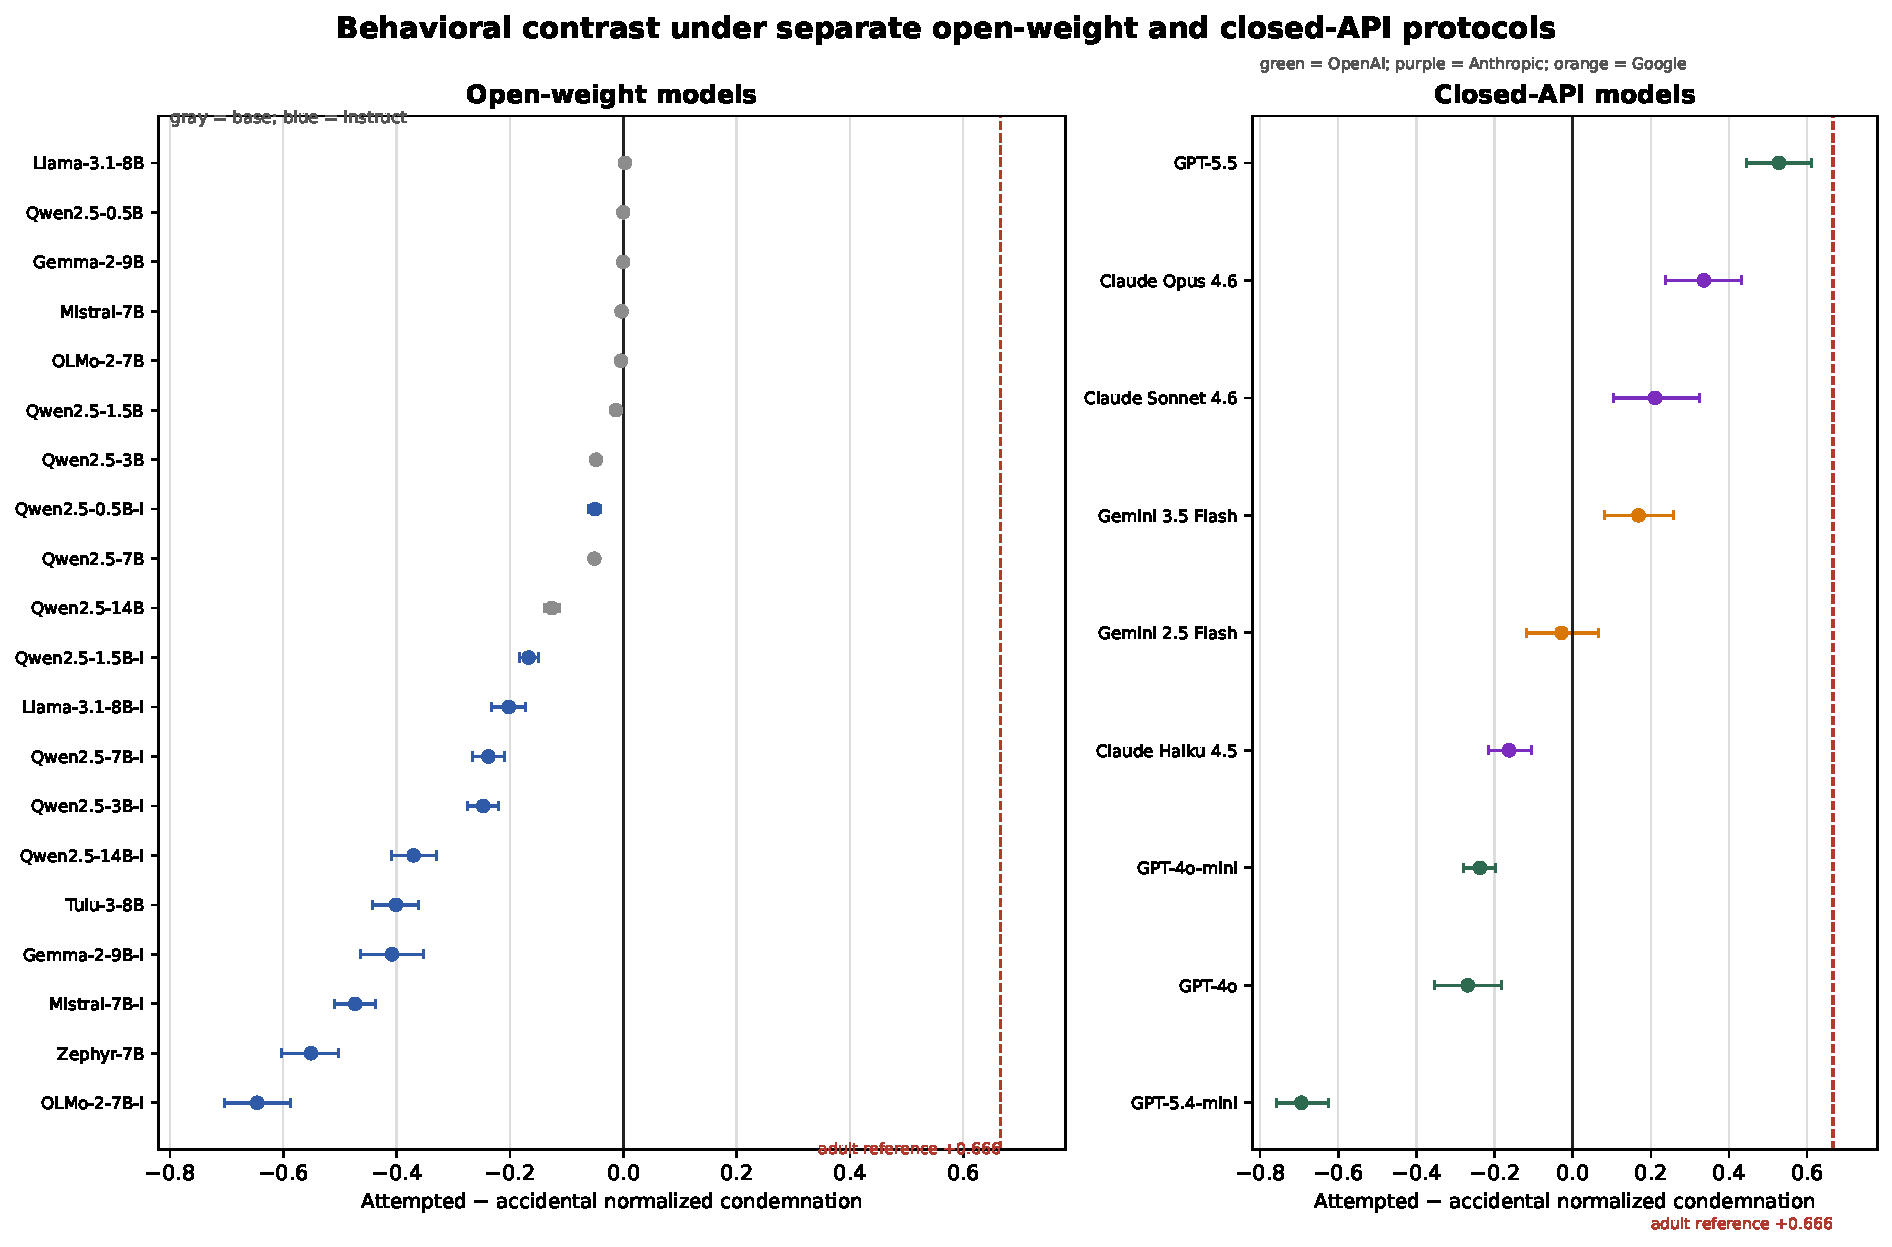
\includegraphics[width=\textwidth]{figures/behavioral_overview.pdf}
    \caption{\textbf{Behavioral attempted-minus-accidental contrast under separate protocols.}
    Positive values place attempted harm above accidental harm.
    The red dashed line is the non-item-matched adult reference ($+0.666$).
    Open-weight estimates use deterministic log-probability expected values over the available post-repair prompt set; closed-API estimates use three templates, five samples, and temperature 1.
    The panels should not be treated as one exchangeable meta-analytic sample.}
    \label{fig:behavior-overview}
\end{figure*}

Prompt analyses further constrain simple model rankings.
Across the six common 1--7 factorial prompts, five of 20 open models changed contrast sign across prompts.
Construct choice explained approximately 0\% of the reported prompt-factorial variance, and a scoring-parity check for 7B instruct models found expected-value and sampling scores correlated above 0.95.
Within the five Qwen base/instruct size pairs, instruction tuning shifted the contrast by approximately $-0.216$ on average ($p\approx0.020$ in the paired test; Wilcoxon $p\approx0.063$).
The separate normalization audit, which covers all nine open base/instruct pairs from five families, found the same direction: the mean instruct-minus-base contrast was $-0.319$ [$-0.345$, $-0.291$] under endpoint scaling, and every pair was negative with an interval excluding zero under endpoint and per-model min--max scaling.
Under within-cell z-scores and ranks the class difference stayed negative but Qwen2.5-14B reversed, so pair estimates are not normalization-invariant, and nine pairs do not establish a universal instruction effect; the model ordering was stable across schemes (Spearman $\rho\geq0.94$ over 34 rater entries).
Item differences beyond the $2\times2$ design were reproducible across instruct models (within-condition split-half 0.83--0.93 across the three sources) but less so across base models (0.36--0.64), and items clustered by outcome (adjusted Rand index 0.88) rather than by intent or source (\cref{sec:supp-normalization}).

\subsection{Explicit false-belief success does not guarantee applied intent weighting}

The six engaged open instruct models scored 0.815--0.985 on hard BigToM false-belief items while producing moral contrasts from $-0.370$ to $-0.646$ (\cref{fig:tom-vs-contrast}).
Thus, every model in this high-false-belief subset occupied the high-explicit/negative-applied quadrant.
This is a within-model coexistence result, not a correlation claim.
The covariate-adjusted all-model regression was bounded but non-significant ($\beta_{\mathrm{ToM}}=-0.379$, $p=0.211$); instruct-only and within-family intervals were too wide for a directional conclusion.

\begin{figure}[t]
    \centering
    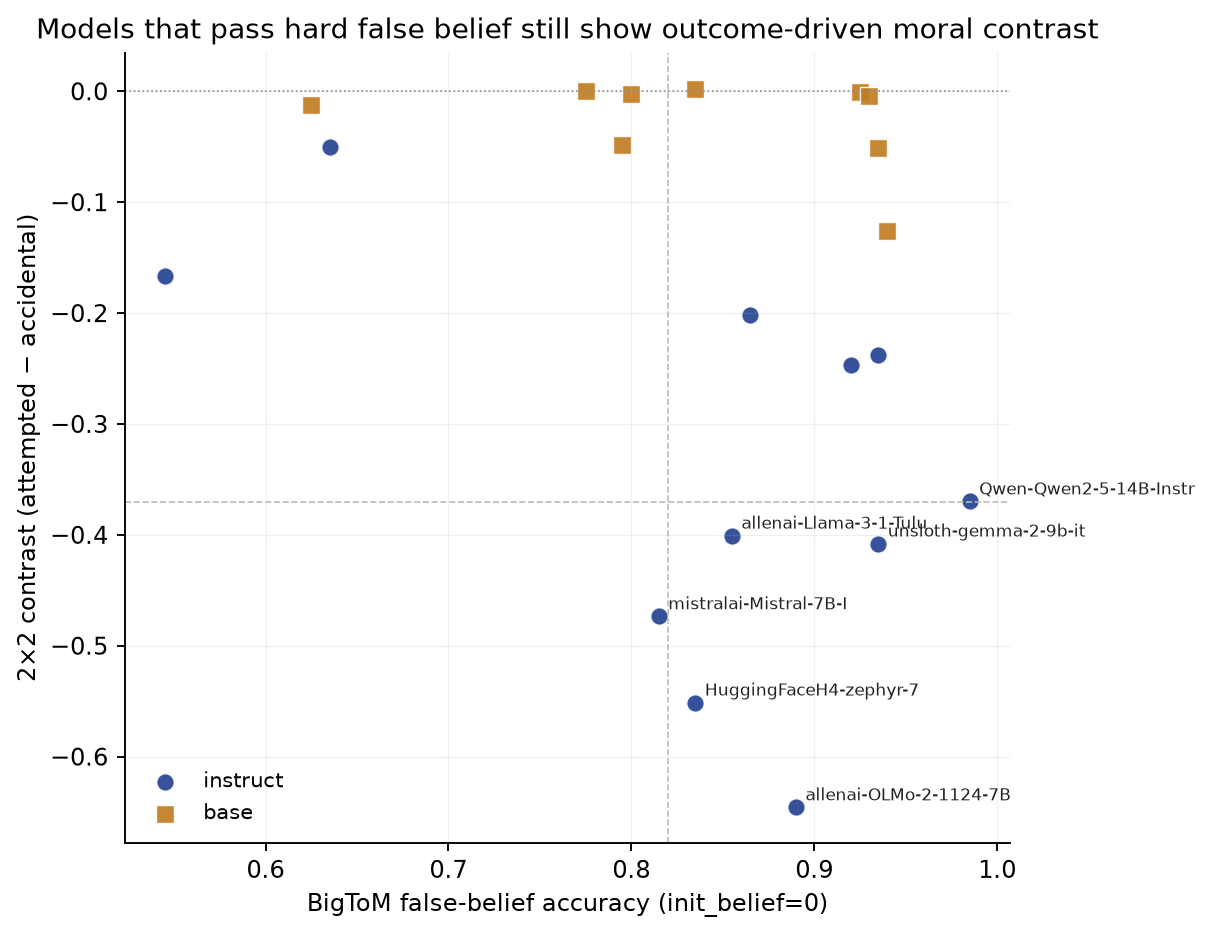
\includegraphics[width=0.72\linewidth]{figures/tom_vs_contrast.png}
    \caption{\textbf{Explicit false belief versus applied moral judgment in open models.}
    Blue circles denote instruct models and ochre squares base models.
    The six engaged instruct models pass the hard false-belief measure while retaining negative moral contrasts.
    No raw regression line is interpreted because both axes covary with model type and size.}
    \label{fig:tom-vs-contrast}
\end{figure}

\subsection{Post-training induces outcome-dominant ratings}

All three public pipelines began near zero and moved negative after supervised fine-tuning (\cref{tab:stages}).
SFT alone shifted OLMo by $-0.5879$, Tulu by $-0.2651$, and Zephyr by $-0.1487$.
It accounted for 85.4\%, 65.4\%, and 27.0\% of each pipeline's total base-to-final shift, respectively; Zephyr's DPO stage accounted for the remaining 73.0\%.
Therefore SFT was sufficient in all three cases, but the dominant stage was recipe-dependent.
Across all non-base stages, $\outcomebeta/\intentbeta$ ranged from 3.0 to 7.7.


\subsection{Intent is decodable, but measured representational differences do not predict use}

At the final story token, peak intent decoding ranged from approximately 0.67 to 0.88 across the eight core checkpoints, while outcome decoding was approximately 0.98--1.00.
At the belief-clause endpoint, intent decoding was 0.90--0.98 against a span-matched TF--IDF baseline of 0.591.
The average intent-minus-outcome gap over their respective span-matched baselines was $+0.087$ (8/8 models, sign-test $p=0.0078$).
Outcome was also decodable at this endpoint (0.79--0.92 in the same checkpoints; 0.70--0.87 at a fixed relative depth of 0.65 across 14 checkpoints, against a word TF--IDF baseline of 0.631 on the 290-story clause-masked set; all $p=0.001$).
That signal is a readout of the foreshadowing sentence, not inference about an unstated outcome: when the sentence was deleted, the prefix became byte-identical across outcome partners and decoding fell to chance (0.496--0.504 at every saved layer in all six models tested; \cref{sec:supp-foreshadow}).
Probes still exceeded TF--IDF on the original prefix by 0.07--0.24, so the foreshadowed content is encoded beyond bag-of-words features.
This analysis concerns outcome only; intent decoding at the same token and depth was 0.85--0.96.
The belief-endpoint results therefore support semantically generalized encoding of stated information, not anticipation of outcomes or a clean early-intent/late-outcome sequence.

Intent decoding also generalized across rating prompts.
At the final prompt token, probes trained with every template of one construct held out reached peak held-out accuracies of 0.64--0.83 in the Qwen2.5-7B and Llama-3.1-8B base and instruct models (all $p=0.001$), exceeding a full-prompt TF--IDF baseline of 0.600 by $+0.04$ (Llama base) to $+0.23$; at the fixed depth, Llama base did not exceed it (0.601).
Transfer between single templates was weaker, especially in base models (0.56--0.57 at the fixed depth, below the 0.596 TF--IDF baseline for that split), whereas instruct models reached 0.58--0.71 (\cref{sec:supp-templates}).
With two pairs, this supports construct-general intent information in these models, not a general base/instruct difference.

Token-wise decoding refines the timing (\cref{fig:time-decoding}).
Intent rose from chance in the background stage to 0.95--0.98 at the end of the belief clause, above the shuffle band and a same-prefix TF--IDF curve (at most 0.64), declined by 0.16--0.21 over the later action and outcome bins, and partially recovered at the final token (0.81--0.86).
Outcome was already decodable at 0.87--0.90 at the end of the background stage, where the foreshadowing sentence falls, drifted down through the belief and action stages, and reached 0.99--1.00 in the outcome clause.
In the RDM regression, the intent coefficient rose from 0.08--0.16 in the background to 1.57--1.69 in the belief stage; the outcome coefficient was 1.46--1.57 in the background and 1.86--1.92 in the outcome stage; and the conjunction coefficient stayed between $-0.12$ and $+0.08$, consistent with additive intent and outcome geometry.
Base and instruct curves were nearly indistinguishable within each family, although their behavioral contrasts differed by $-0.18$ to $-0.69$ under endpoint scaling.

\begin{figure*}[t]
    \centering
    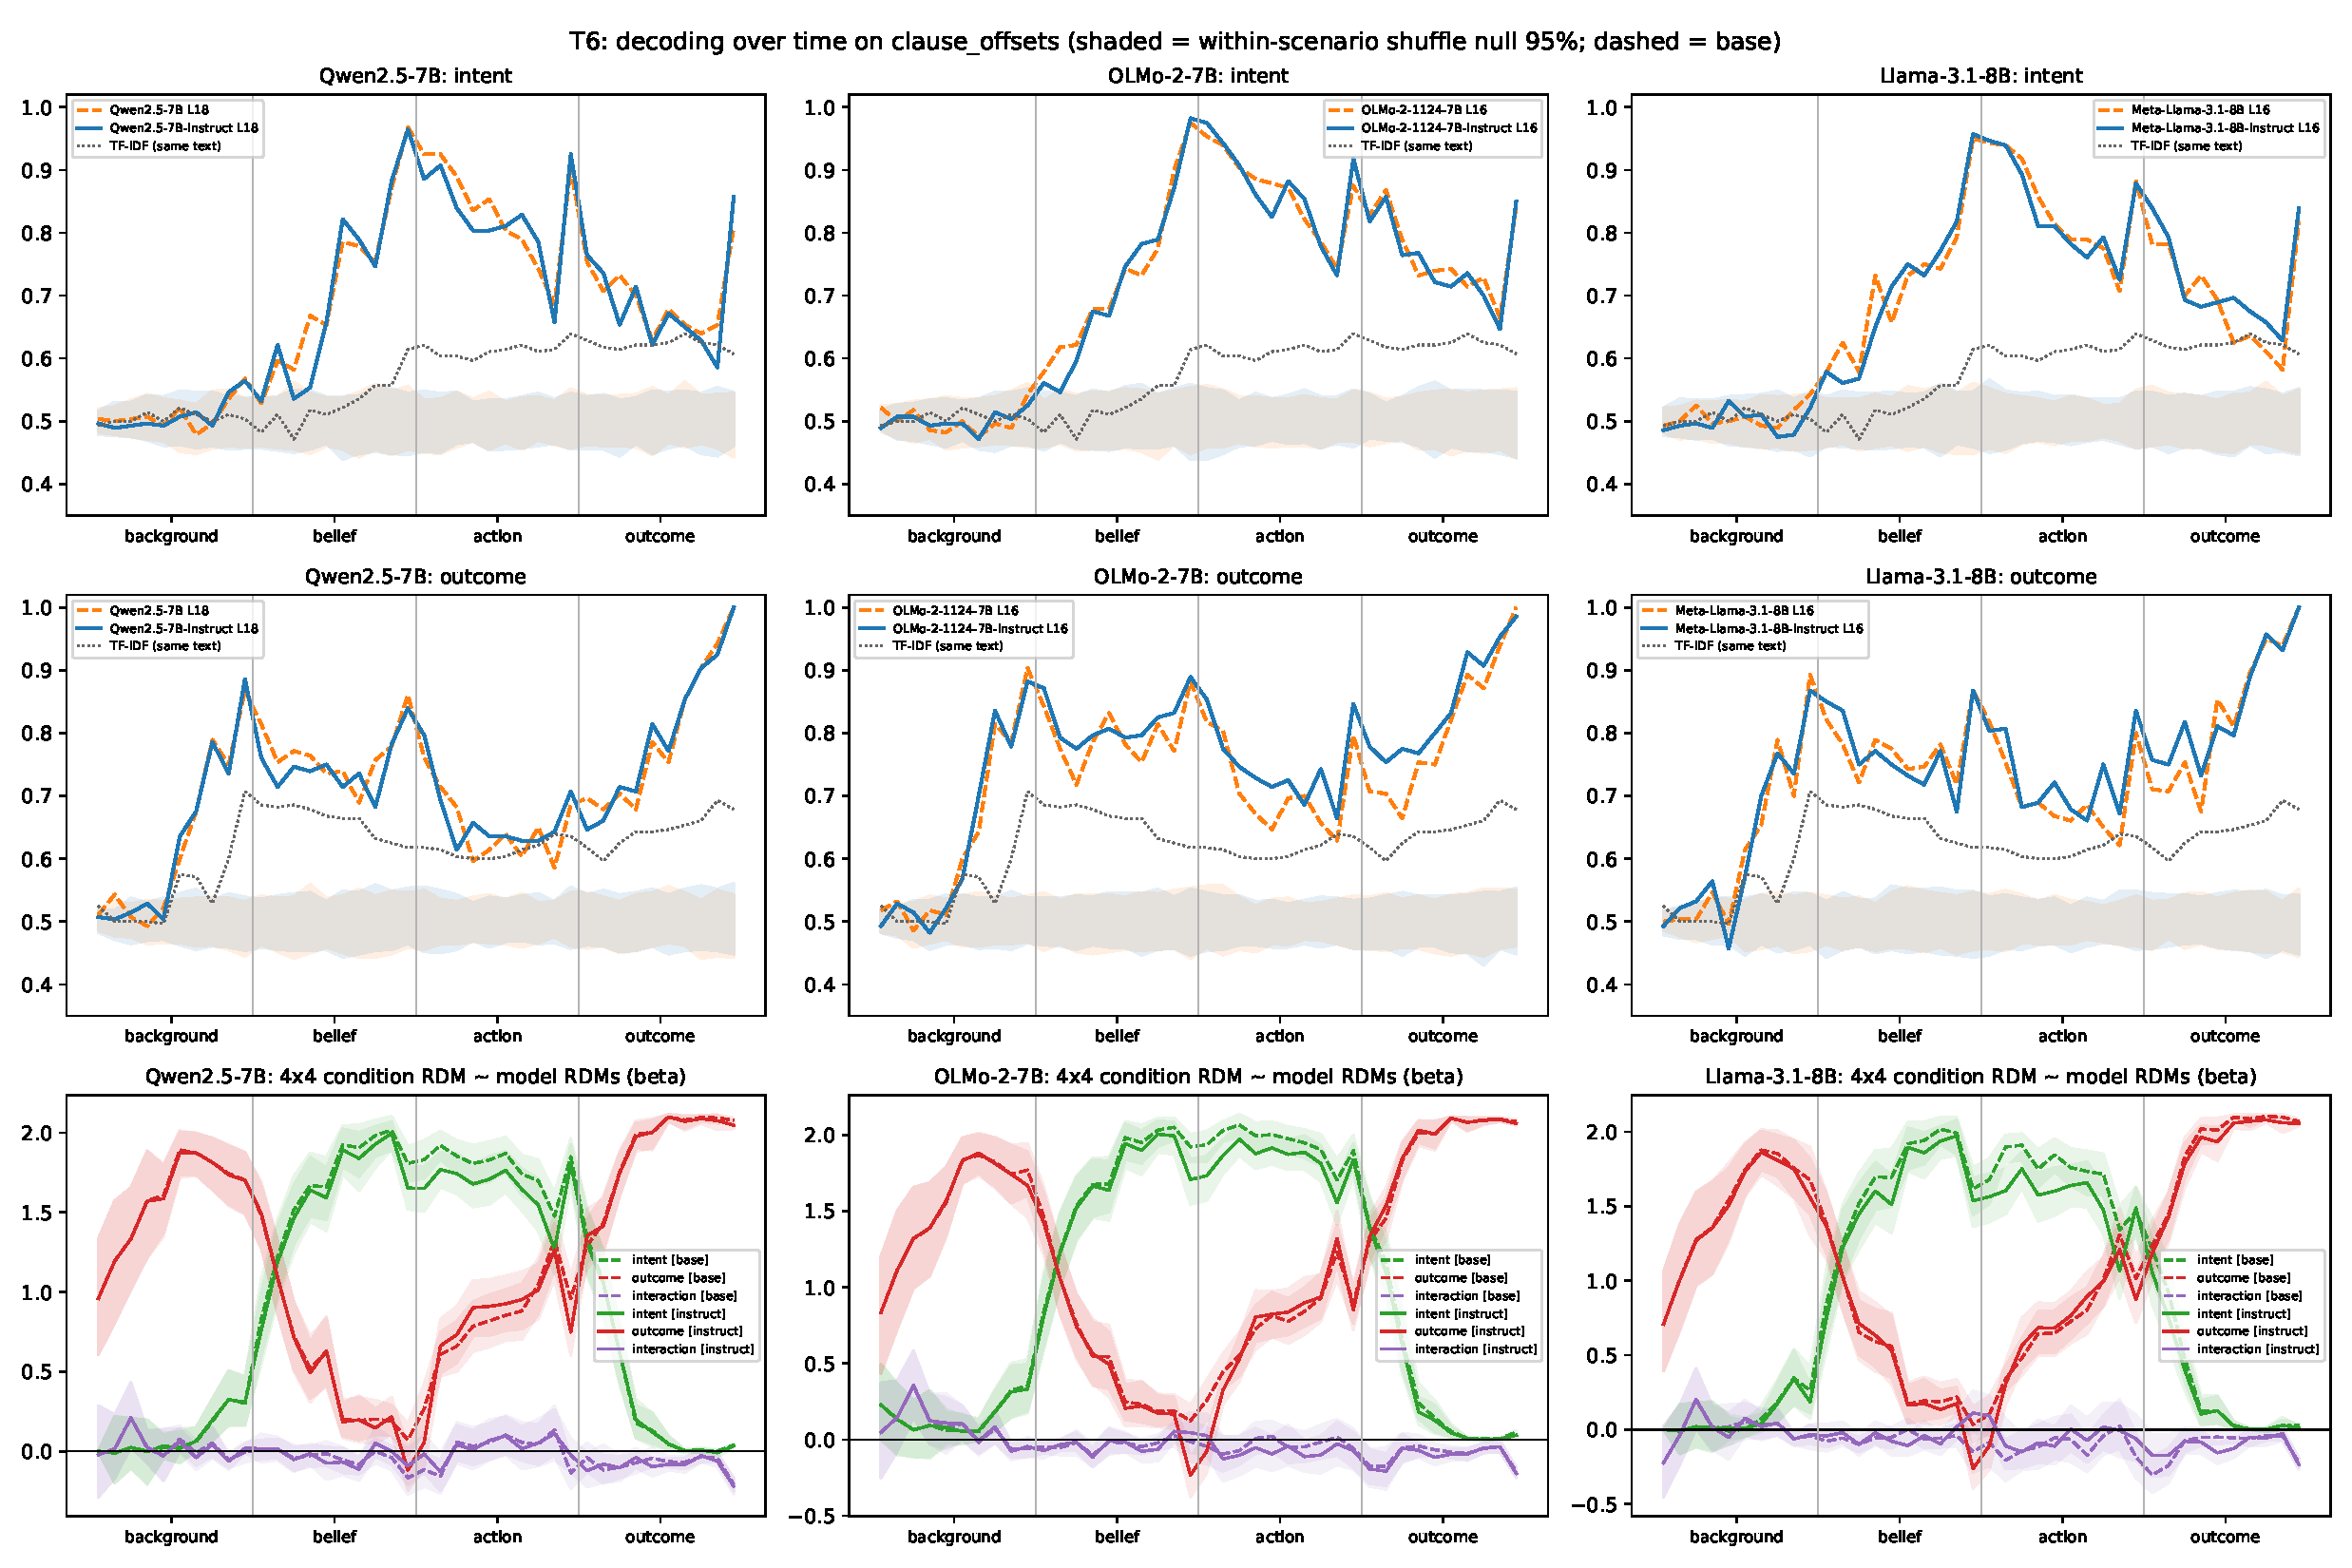
\includegraphics[width=0.86\textwidth,trim=0 0 0 28,clip]{figures/fig_T6_time_decoding.pdf}
    \caption{\textbf{Token-wise decoding along the story.}
    Rows show intent decoding, outcome decoding, and four-condition RDM regression coefficients at 40 positions (ten bins per stage) for three base/instruct pairs at a fixed layer per family (Qwen 18, OLMo 16, Llama 16; the Llama layer was assumed rather than selected).
    Shading is the 95\% within-scenario shuffle band (100 shuffles); dotted lines are TF--IDF on the same prefix; dashed lines are base models.
    Early outcome decoding reflects the foreshadowing sentence (\cref{sec:supp-foreshadow}).
    Trajectories were extracted without chat formatting.}
    \label{fig:time-decoding}
\end{figure*}

Decodability did not imply behavioral coupling.
The pooled item-level intent-margin slope was $+0.0619$ [${-0.1463},+0.2701$], excluding the pre-stated meaningful slope of $+0.30$; the matched definition was $+0.0291$ [${-0.1649},+0.2231$].
Across 28 model pairs, RSA geometry--behavior correspondence was $r=+0.098$ [${-0.31},+0.46$].
The model-level probe--behavior association was too imprecise to interpret and is not a headline result.

Two secondary analyses were inconclusive: the pre-registered RDM variance partition was undecidable because lexical-control gating excluded 36/36 target cells, and checkpoint-stage RSA ($\rho=+0.870$, $n=6$, 95\% interval $[+0.200,+1.000]$) was withdrawn as underpowered.

\begin{figure*}[t]
    \centering
    \begin{subfigure}[t]{0.49\textwidth}
        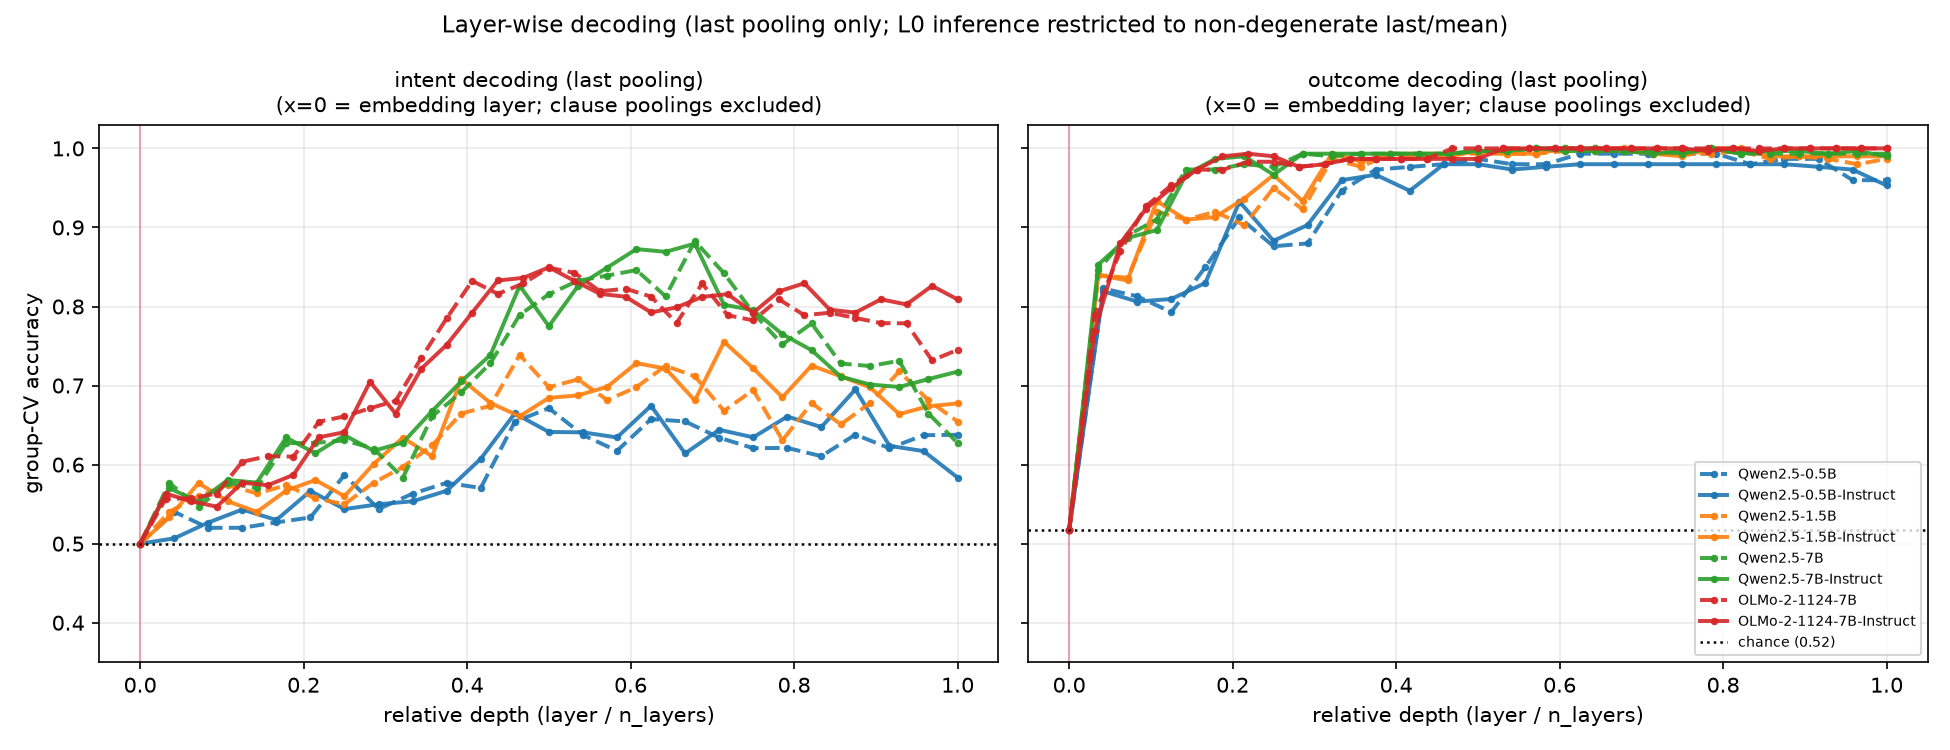
\includegraphics[width=\linewidth]{figures/layerwise_curves.png}
        \caption{Layerwise linear decoding.}
    \end{subfigure}
    \hfill
    \begin{subfigure}[t]{0.49\textwidth}
        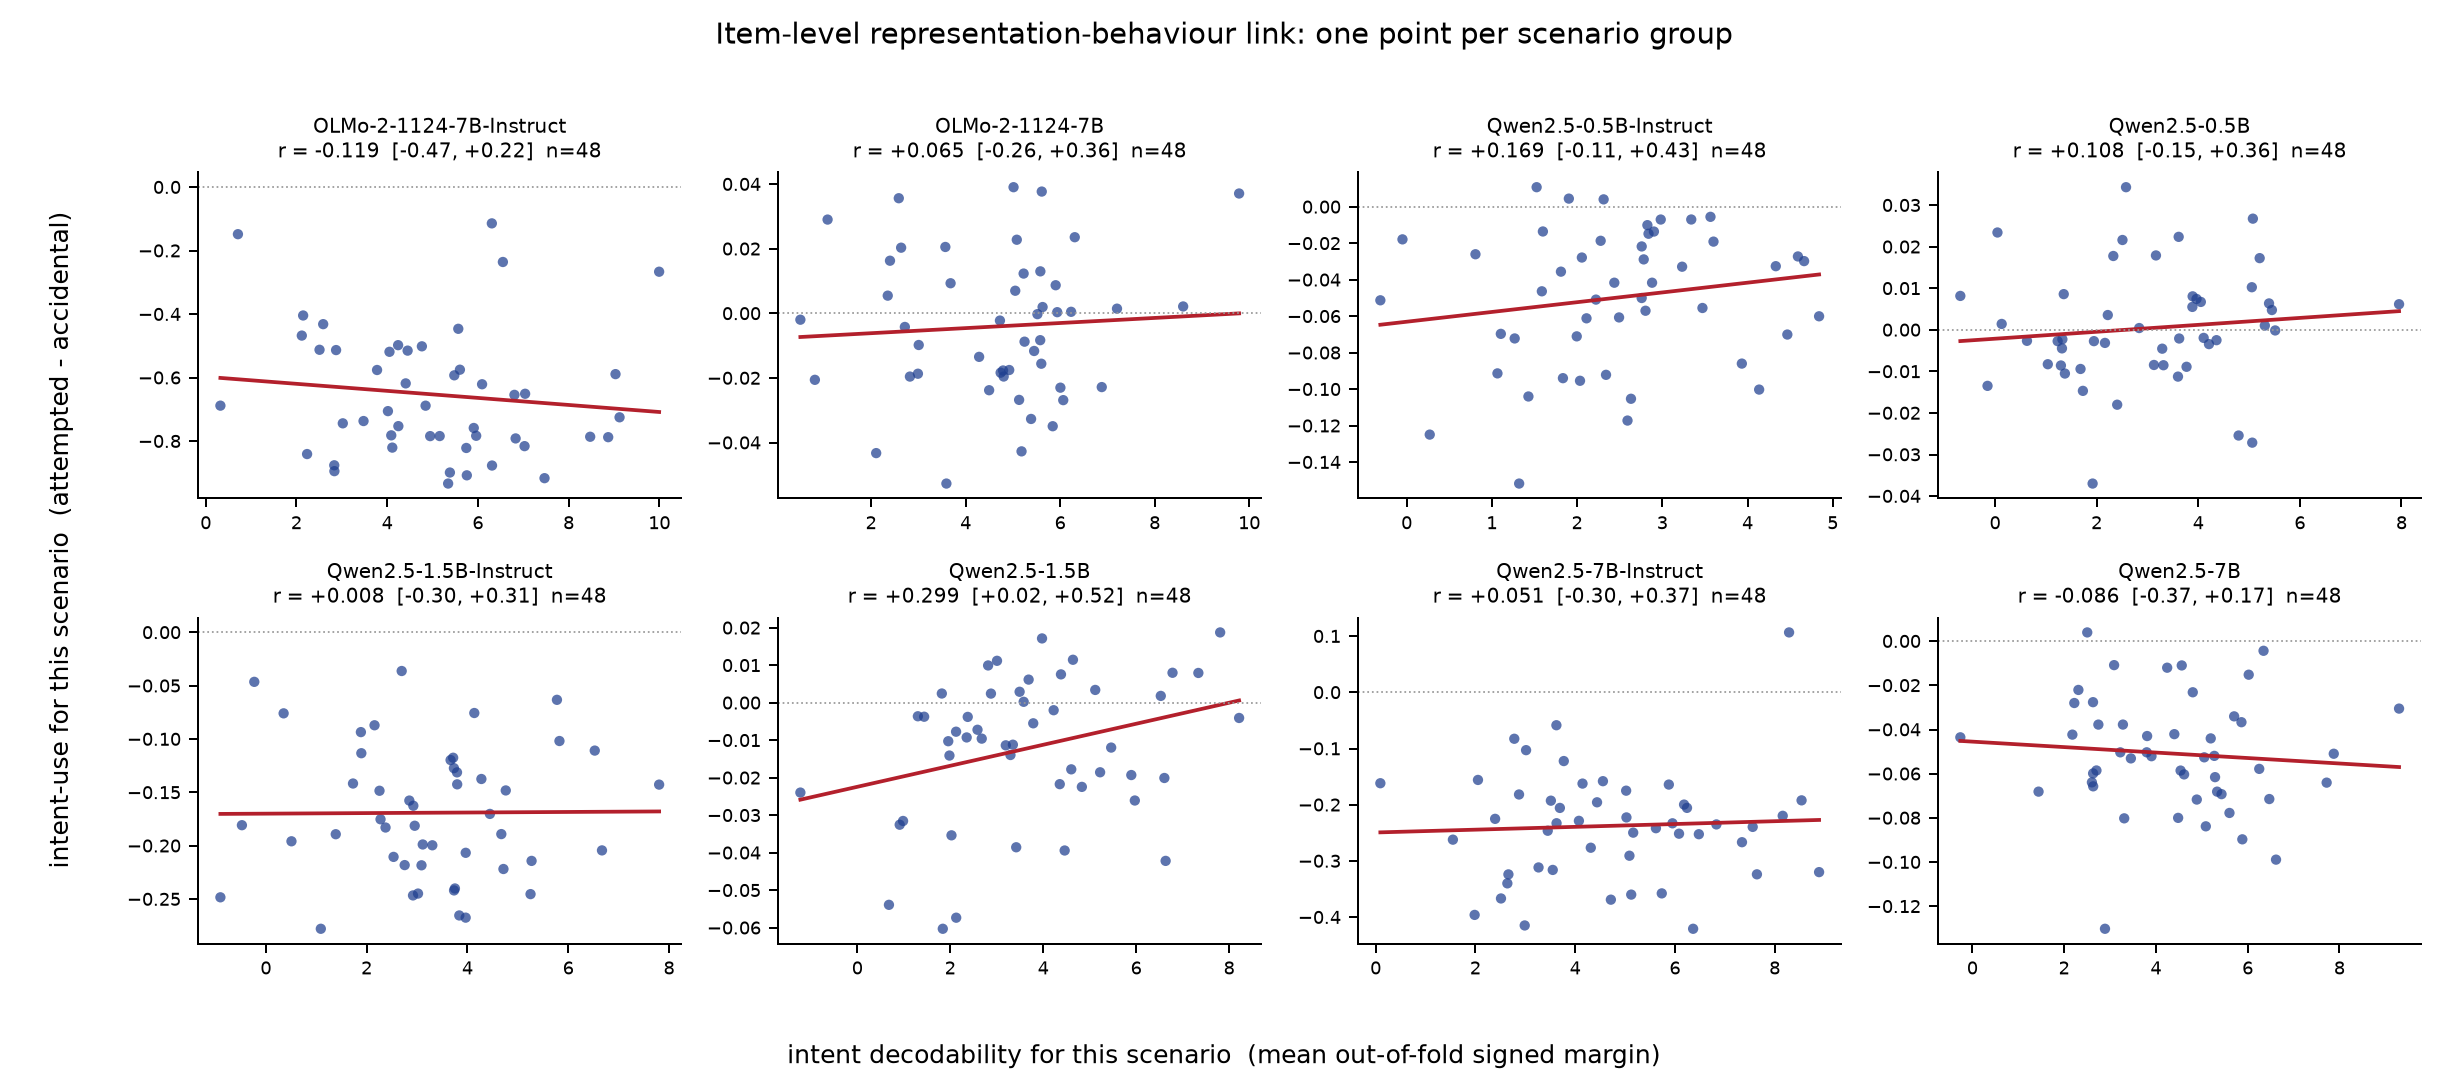
\includegraphics[width=\linewidth]{figures/item_level_dissociation.png}
        \caption{Item-level representation--behavior link.}
    \end{subfigure}
    \caption{\textbf{Representation without a corresponding behavioral link.}
    Intent and outcome are linearly decodable, but item-level intent margins do not predict intent-sensitive ratings at the pre-specified effect size.
    All folds respect scenario groups.}
    \label{fig:probes-link}
\end{figure*}

\subsection{Interventions separate readable intent from outcome-dominant readout}

\paragraph{Additive steering.}
At coherent coefficients, the probe-weight intent direction changed $\contrast$ by at most 0.0128 in OLMo and 0.0155 in Qwen.
The outcome-direction positive control changed the same contrast by 0.2319 and 0.2592.
The manipulation check showed that intent steering moved downstream probe margins by 3.2--7.2 SD in magnitude and drove held-out intent decoding from approximately 0.89 to 0.50, while the rating contrast remained nearly fixed.
Layer sweeps supported the narrow claim at the peak-intent layer and deeper, where direction specificity was resolvable; shallow layers were uninformative.
This bounds the tested linear, all-token, single-layer intervention and does not exclude other intent encodings.

\paragraph{Model explanations.}
Unprompted explanations named belief or intent in 81.5\% (OLMo) and 69.1\% (Qwen) of stories, yet within those subsets $\outcomebeta/\intentbeta$ was 5.7 and 12.2 and both contrasts stayed negative; because explanations followed the rating, this is output-level dissociation, not a causal account (\cref{tab:prose}).

\paragraph{Prompt curriculum.}
At the pre-registered top level, only three of six models exceeded the $+0.15$ improvement criterion, below the required four.
Five of six top-level improvements were primarily reductions in accidental blame rather than increased condemnation of attempts.
Intent-led movement occurred in two of six models and only under the principle-alone ablation.
The result does not support ``unreachable by steering but reachable by prompting''; it supports partial, inconsistent prompt sensitivity.

\begin{figure*}[t]
    \centering
    \begin{subfigure}[t]{0.49\textwidth}
        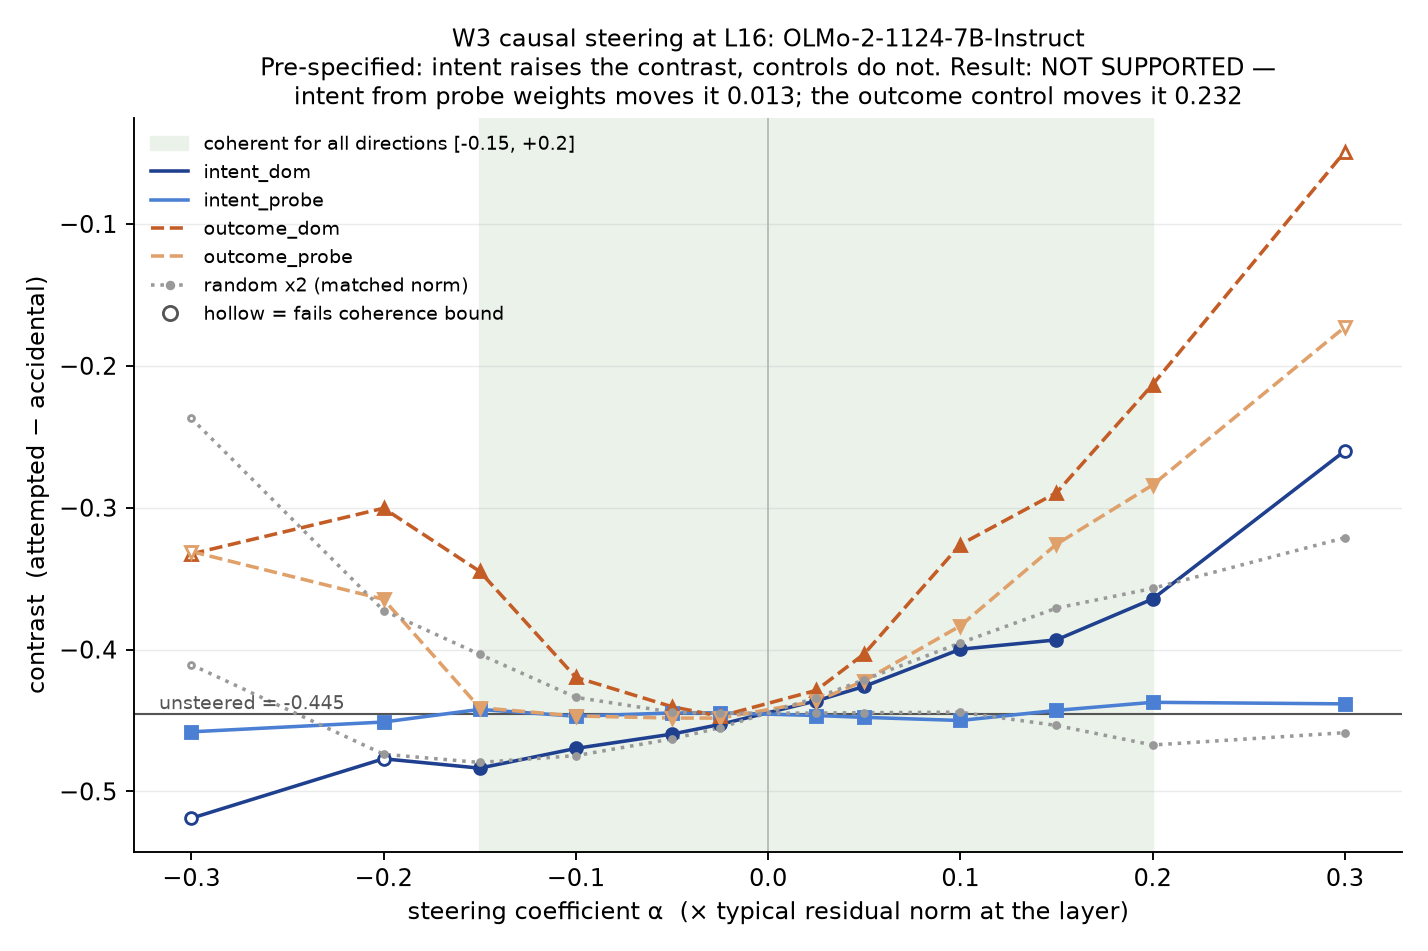
\includegraphics[width=\linewidth]{figures/w3_steering_OLMo.png}
        \caption{OLMo additive steering.}
    \end{subfigure}
    \hfill
    \begin{subfigure}[t]{0.49\textwidth}
        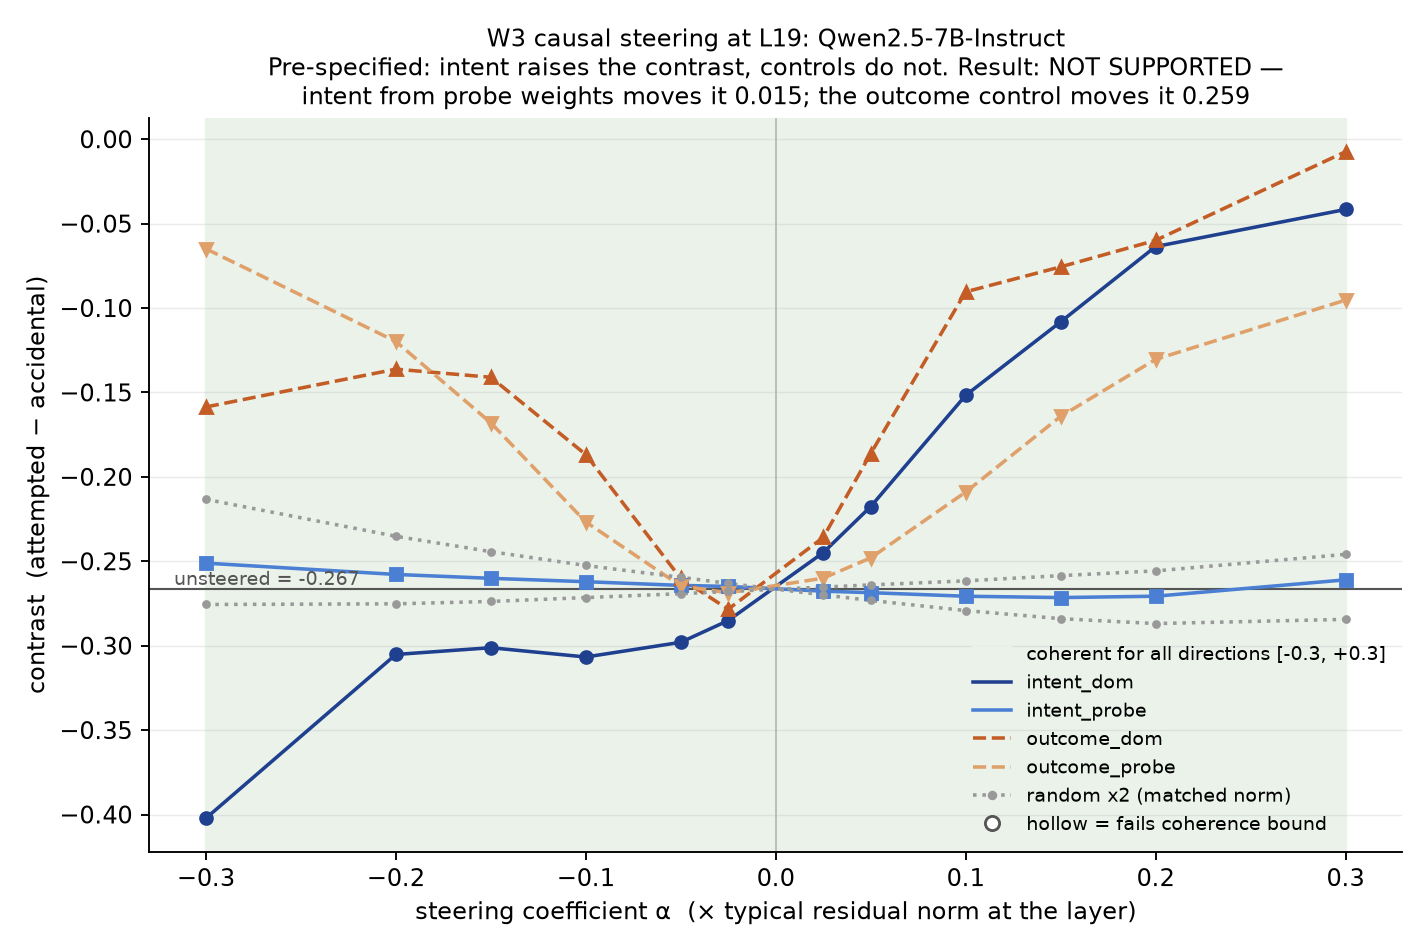
\includegraphics[width=\linewidth]{figures/w3_steering_Qwen.png}
        \caption{Qwen additive steering.}
    \end{subfigure}
    \caption{\textbf{Probe-weight intent steering is behaviorally small relative to the outcome control.}
    Difference-of-means directions can move all four cells toward a scale ceiling and are not interpreted as selective intent reweighting.}
    \label{fig:steering}
\end{figure*}

\paragraph{Outcome erasure.}
Rank-one outcome erasure produced a recovery signature in OLMo.
Here, $\Delta\contrast=+0.3182$ and cell-spread retention was 0.5124.
Qwen also recovered ($+0.2312$; retention 0.6697).
Tulu moved most ($+0.3480$) but retained only 0.3753 of its cell spread.
It fell below the pre-registered 0.50 boundary and was classified as collapse.
The headline is therefore recovery in two of three models.

Specificity is bounded.
The original E5a control failed in Qwen: a matched-norm scenario perturbation moved the contrast $+0.1345$, a 1.72$\times$ separation below the required 2$\times$, so outcome is the most effective direction found, not the only effective perturbation.
A differently specified E6 control---orthogonalized nuisance erasure with no over-projection---was inert in all three models (maximum $|\Delta\contrast|=0.0160$) and produced 9.9$\times$, 22.3$\times$, and 24.6$\times$ separation.
E7b then split by model: OLMo was A-shaped, with recovery surviving removal of the scenario-aligned component, and Qwen was void because its matched positive control failed.
Tulu followed the pre-registered falsifier branch, although its test arm reached 95\% of the effect floor and the complement cleared it by only 0.0020.
The decision table is retained, but the near-threshold result and cross-model split do not license a pooled outcome-specific mechanism.

\begin{figure*}[t]
    \centering
    \begin{subfigure}[t]{0.32\textwidth}
        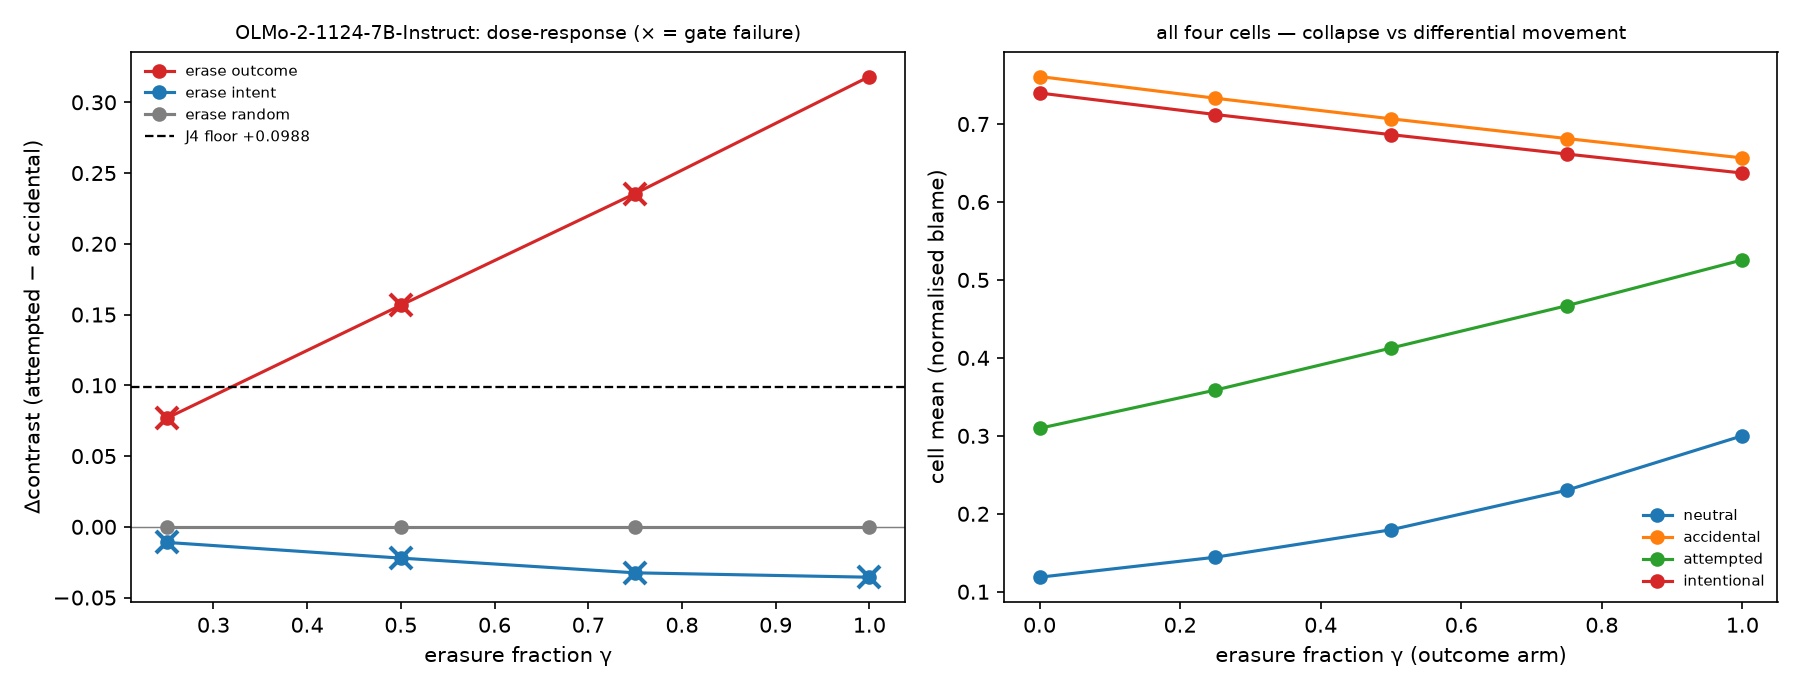
\includegraphics[width=\linewidth]{figures/w8a_OLMo.png}
        \caption{OLMo: recovery.}
    \end{subfigure}
    \hfill
    \begin{subfigure}[t]{0.32\textwidth}
        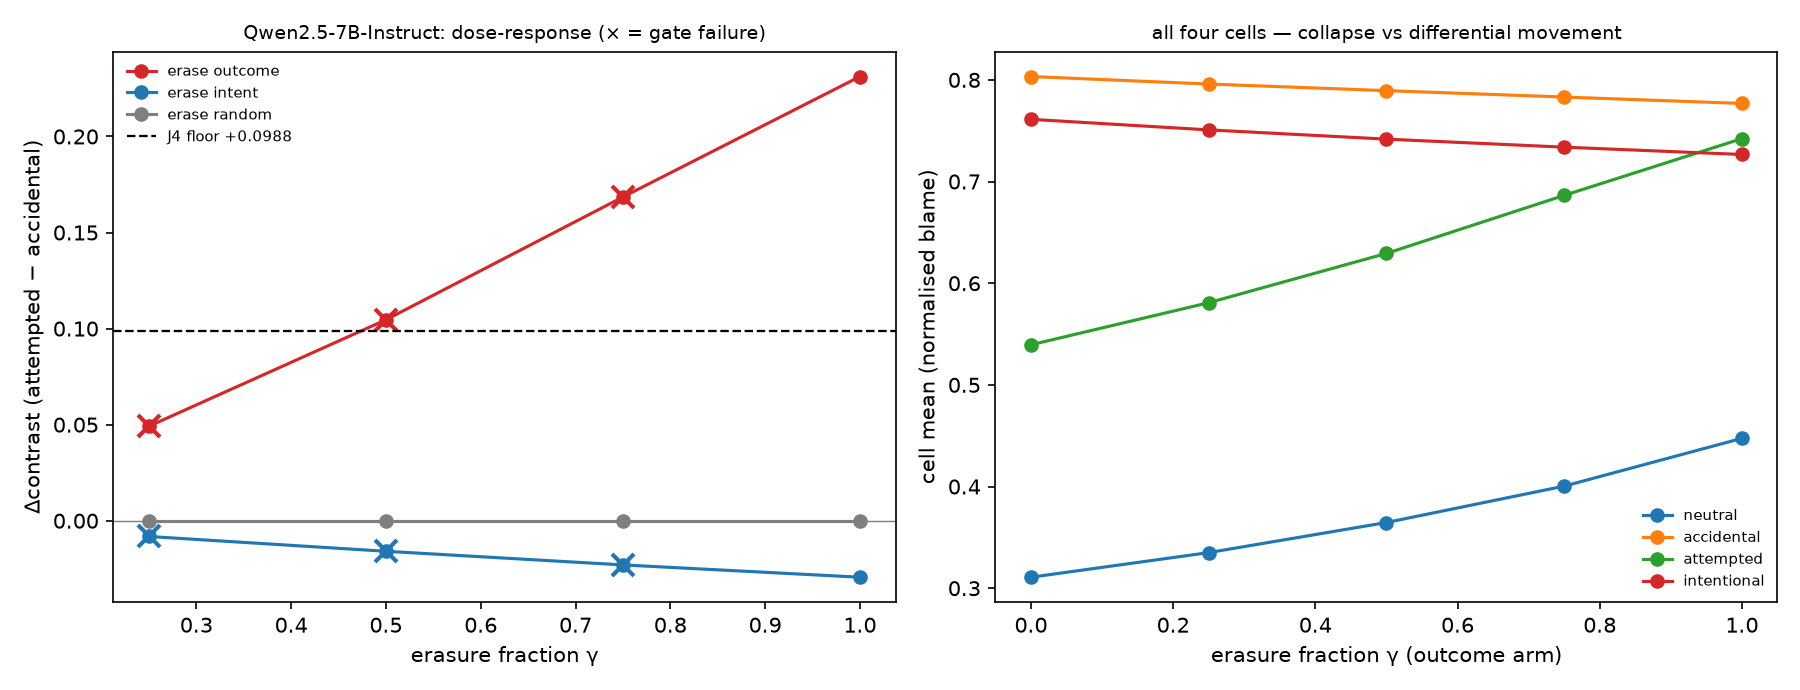
\includegraphics[width=\linewidth]{figures/w8a_Qwen.png}
        \caption{Qwen: recovery.}
    \end{subfigure}
    \hfill
    \begin{subfigure}[t]{0.32\textwidth}
        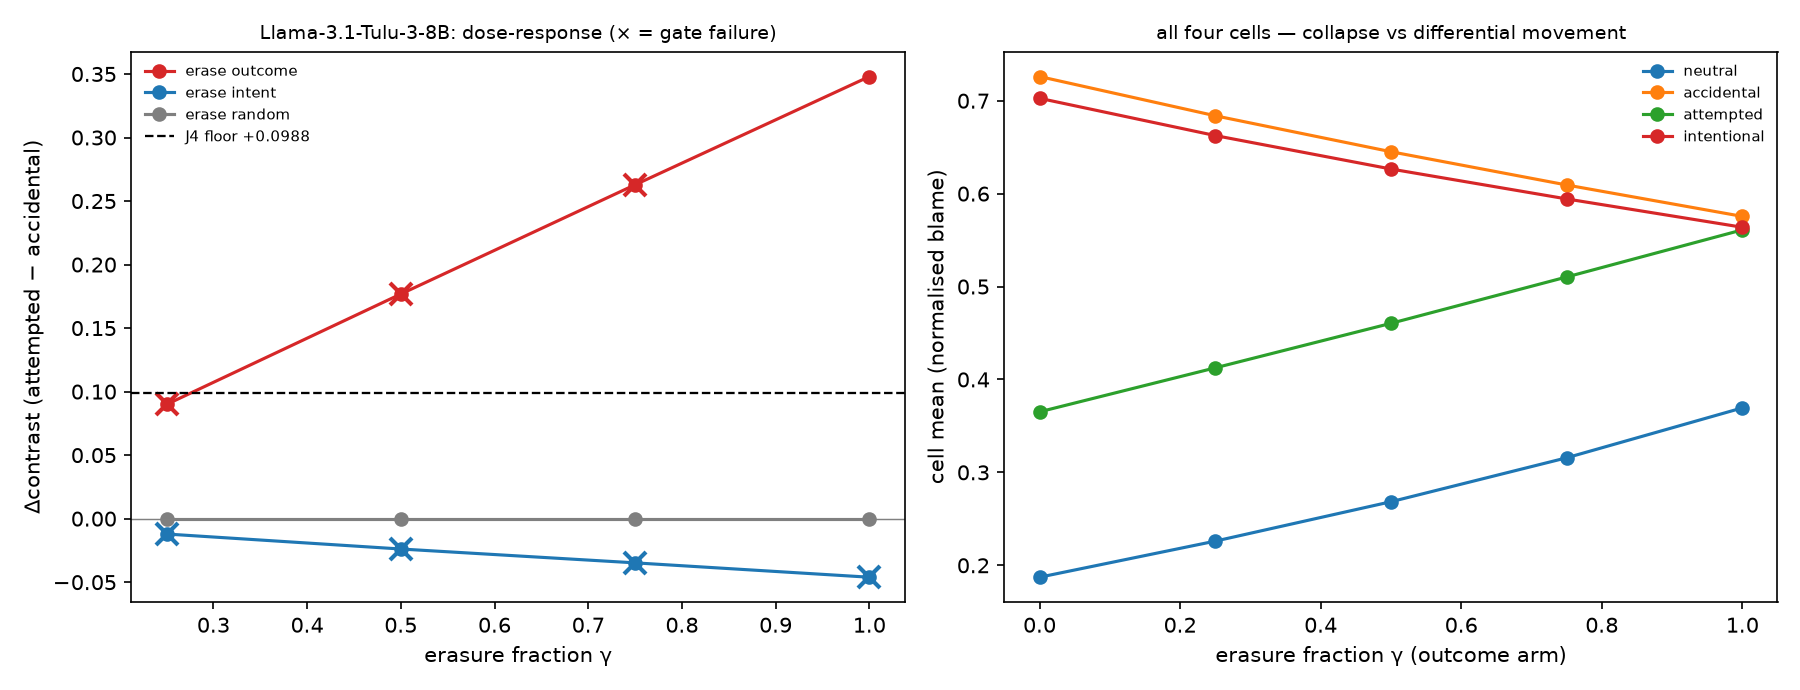
\includegraphics[width=\linewidth]{figures/w8a_Tulu.png}
        \caption{Tulu: collapse at full erasure.}
    \end{subfigure}
    \caption{\textbf{Outcome erasure changes the behavioral contrast, but its interpretation depends on retained cell structure.}
    Only OLMo and Qwen meet the pre-registered recovery signature at the gate-passing dose.}
    \label{fig:erasure}
\end{figure*}

\subsection{Representations emerge during pretraining; gradeable moral ratings do not}

In Pythia-1.4B, the end-of-story geometry became strongly organized by outcome ($\beta$ reached $+0.4899$ at step 143{,}000), while intent stayed near zero at that read position.
At the belief-clause endpoint, intent reached $+0.1042$ and outcome stayed near zero.
Across informative cells, sigmoid fits in log step were preferred to free-breakpoint fits, supporting gradual rather than abrupt representational development.
No Pythia checkpoint crossed the behavioral engagement floor (0/26).

OLMo-2-7B replicated the position-dependent pattern at the final stage-1 revision: intent cleared its null and outcome did not at five of five depths at the belief endpoint; outcome cleared and intent did not at four of five depths at story end.
At depth 0.8, both target factors were inside their null at step 1{,}000 (approximately 5B tokens) and clear from step 2{,}000 (approximately 9B tokens), providing an onset bracket rather than a point estimate.
No stage-1 checkpoint was behaviorally gradeable (0/20); the first gradeable point on the joined OLMo axis was SFT.
As in the probe analyses, the belief endpoint follows the foreshadowing sentence and is therefore not outcome-free.

\begin{figure*}[t]
    \centering
    \begin{subfigure}[t]{0.49\textwidth}
        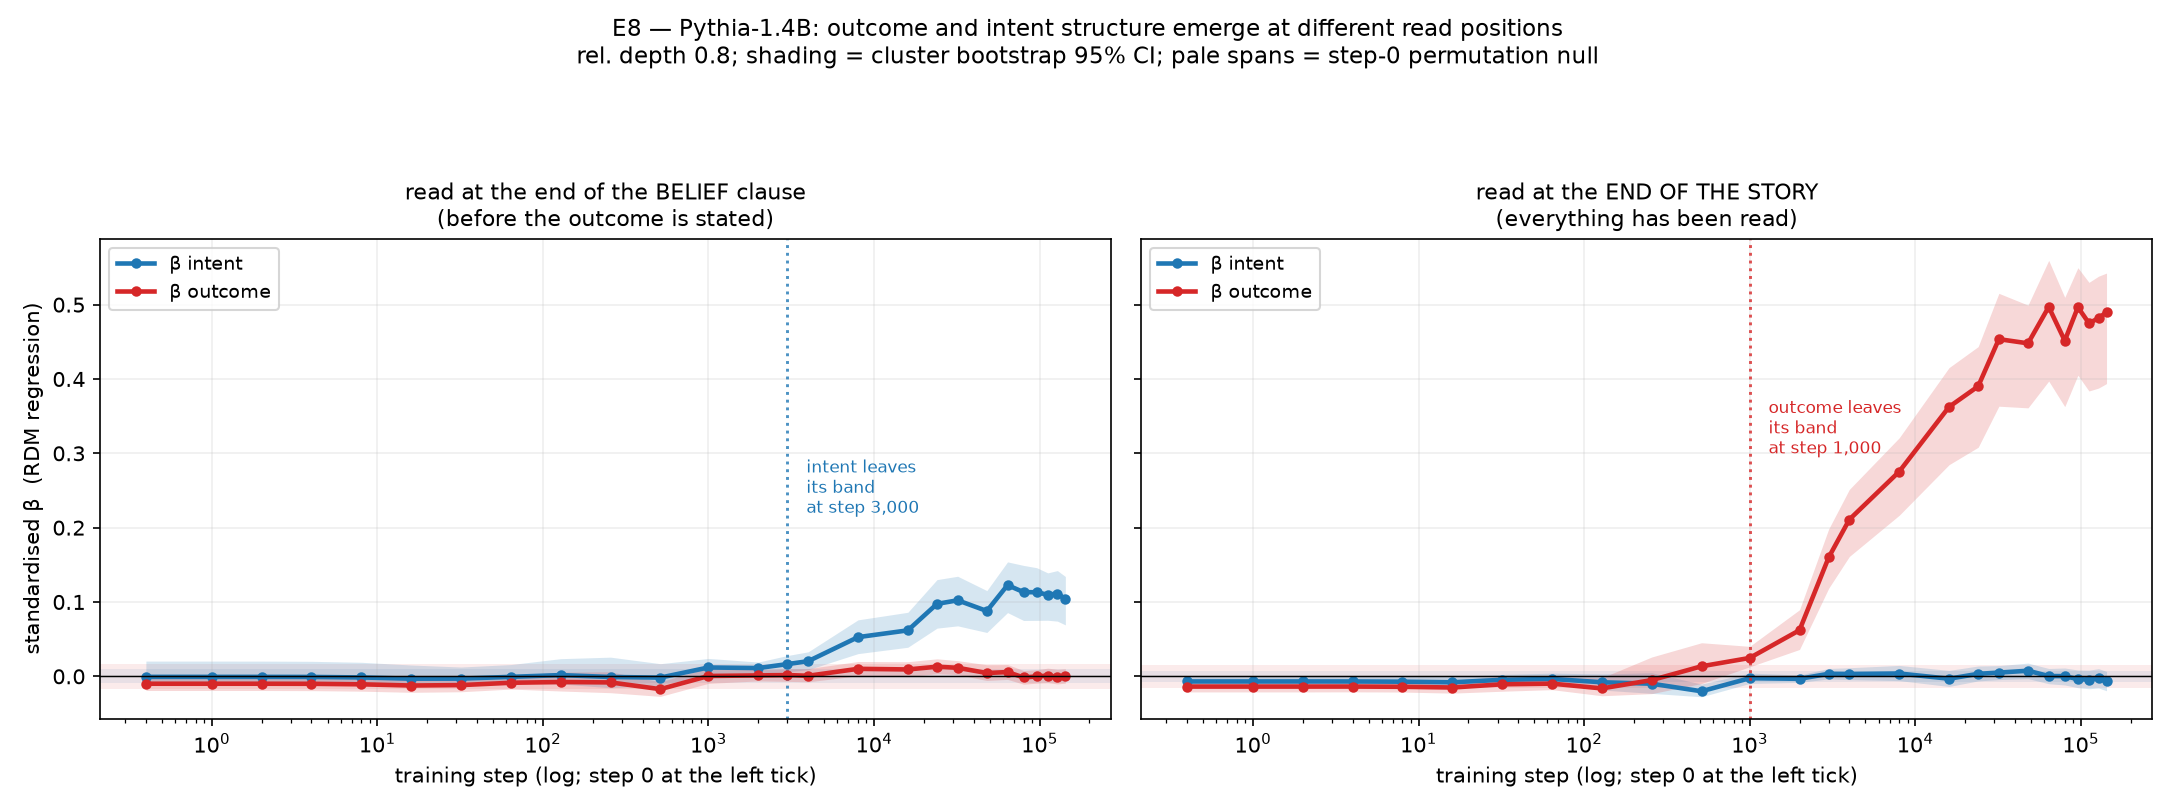
\includegraphics[width=\linewidth]{figures/e8_pythia.png}
        \caption{Pythia-1.4B, 26 checkpoints.}
    \end{subfigure}
    \hfill
    \begin{subfigure}[t]{0.49\textwidth}
        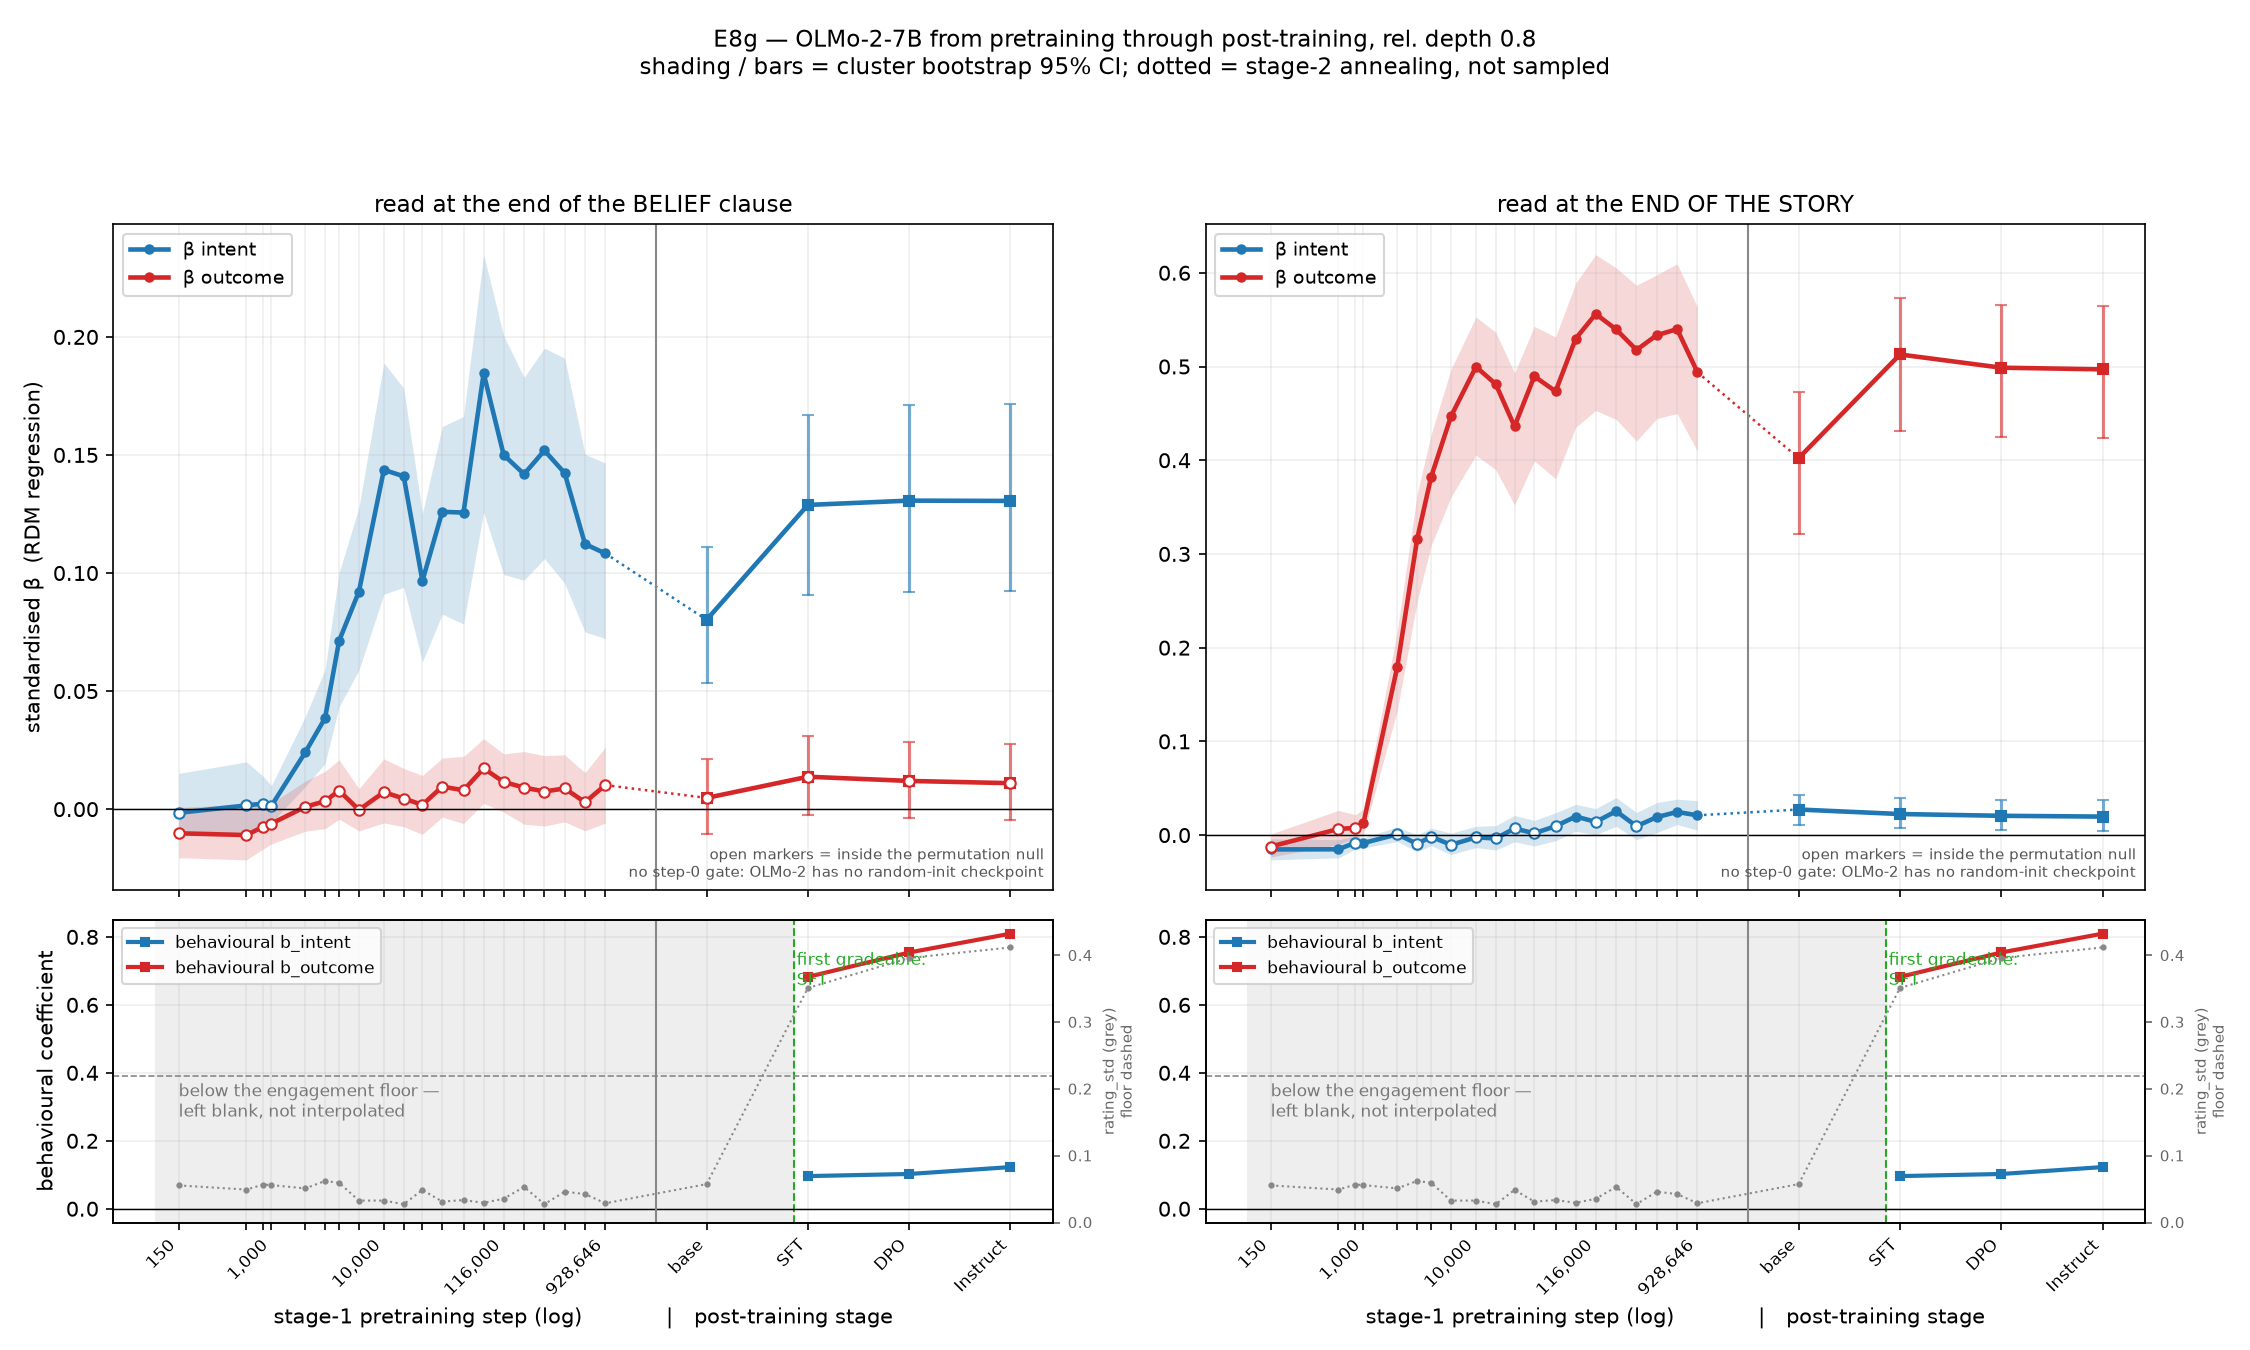
\includegraphics[width=\linewidth]{figures/e8_olmo.png}
        \caption{OLMo-2-7B, 20 stage-1 revisions plus post-training stages.}
    \end{subfigure}
    \caption{\textbf{Smooth, read-position-dependent representational development.}
    Coefficients are standardized RDM regressions, not activations or weights.
    The panels are descriptive trajectories; the OLMo family has no published random-initialization checkpoint, and its stage-2 annealing interval is unsampled.}
    \label{fig:e8}
\end{figure*}

\FloatBarrier
\section{Discussion}

\subsection{Capability, resemblance, and mechanism are different claims}

The central empirical result is a dissociation.
The same engaged open instruct models can answer hard false-belief questions while reversing the adult-reference ordering in graded moral judgment.
Intent is linearly readable, yet measured intent margins and representational geometry do not predict behavioral reliance at the pre-specified scales.
Additive manipulation of the readable intent direction has little behavioral effect where an outcome control is effective.
Outcome erasure produced a more intent-sensitive profile in two models, showing that changing one linearly defined outcome component can alter the readout.
The third model's collapse and the specificity-control split do not establish suppression, a model-general mechanism, or an outcome-unique causal direction.

These observations do not show that the models lack all ToM-like computation.
They show that explicit benchmark success is insufficient evidence for stable, human-reference use of mental-state information in this downstream task.
Nor does a positive closed-model contrast establish a human mechanism: GPT-5.5 and three other closed models more closely match the reference direction behaviorally, but internal evidence is unavailable and the human anchor is not item-matched.
Capability, behavioral resemblance, and mechanism must therefore be reported separately.

\subsection{What the results do and do not say about pattern association}

The results are inconsistent with treating one explicit benchmark score as a sufficient explanation of reusable social reasoning.
They do not, however, identify ``pattern association'' and ``reasoning'' as mutually exclusive mechanisms, and they do not prove that one generated any individual response.
The controlled factorial, prompt tests, held-out scenario groups, cross-task comparison, and intervention results constrain simple benchmark memorization accounts.
They still permit distributed, nonlinear, task-conditioned, or instruction-specific computations.
Two follow-up results sharpen this boundary: intent decoding transferred to held-out rating constructs, arguing against a purely template-specific intent code in the two tested pairs, whereas early outcome decodability was traceable to a single foreshadowing sentence and reflects encoding of stated text rather than prediction.
The appropriate conclusion is methodological: evidence for ToM-like capability should require generalization and information use, not only production of a familiar answer.

\subsection{Learning and post-training}

The pretraining trajectories show that structured intent and outcome geometry can arise smoothly before the model provides a usable graded rating.
In OLMo, the first gradeable point is SFT, and the three-family dissection shows SFT is sufficient to induce the negative contrast in each public pipeline.
However, Zephyr's dominant shift occurs at DPO, so the locus is recipe-dependent.
This combination argues against a single universal ``alignment stage'' account.
It instead suggests that pretraining supplies structured variables and post-training determines whether and how a rating head or prompted continuation expresses them.
Consistent with this, token-wise decoding curves were nearly identical for base and instruct models in three families, while a 20-model variance decomposition assigned the largest unique share of rating variance (8.6\%) to the condition $\times$ base/instruct interaction.
In two pairs, base-model ratings barely changed when the story was replaced by the agent's name alone (mean absolute change 0.06 versus 0.29 for instruct models; difference $+0.24$ [0.22, 0.25]; \cref{sec:supp-ablation}).
That interpretation remains descriptive because the checkpoint sets differ by family and recipe and the ablations cover only two pairs.

\subsection{Implications for evaluation and industry standards}

A robust ToM evaluation should report at least four layers:
\begin{enumerate}[leftmargin=*]
    \item \textbf{Explicit inference:} performance on held-out, perturbation-tested mental-state questions.
    \item \textbf{Applied behavior:} factor weights and full cell profiles in downstream prediction or judgment.
    \item \textbf{Robustness:} prompt, scale, sampling, family, and checkpoint sensitivity, with failed measurements kept missing.
    \item \textbf{Mechanistic evidence where access permits:} group-controlled probes, representation--behavior links, positive-control interventions, and specificity controls.
\end{enumerate}
For closed models, the fourth layer may be unavailable; the correct response is to label the evidence behavior-only rather than infer hidden mechanisms from output.
This tiered procedure is more informative than a single pass rate and makes version-to-version changes auditable.

\subsection{Methodological innovations and research difficulties}

The principal methodological innovations are integrating explicit ToM accuracy with a graded cognitive-science factorial; separating decodability, predictive linkage, and causal intervention; connecting pretraining trajectories to public post-training stages with continuous representational metrics; preserving pre-registered falsifiers, failed controls, and missing measurements in the claim boundary; and auditing stimulus parsing, duplicate groups, scale normalization, and stimulus text such as foreshadowing as part of the scientific result.
These are innovations of integration and test procedure; priority over every component method is not claimed.

The principal research difficulties are construct validity, non-item-matched human references, lexical realization of the manipulated factors, correlated nuisance structure, effective sample size, heterogeneous model-access protocols, and the limited number of models for expensive interventions.
The project also illustrates a practical difficulty in model science: model and API generations can change faster than a complete mechanistic study.
The positive closed-model results narrow the universal behavioral claim while strengthening the need to separate current behavior from mechanisms established in older open models.

\section{Limitations}

\begin{enumerate}[leftmargin=*]
    \item \textbf{Open-model scope.} The largest open model is 14B and half of the 20-model roster is Qwen2.5. No claim is made about all frontier-scale open models or family generality.
    \item \textbf{Human references.} Adult means come from a different 12-scenario set and child bands are digitized, use a different measure, and cover only attempted and accidental cells. The ladder is descriptive, not item-matched ground truth.
    \item \textbf{Cross-cultural axis.} The ten-society comparison uses intentional-minus-accidental at constant harm, not the headline attempted-minus-accidental contrast.
    \item \textbf{Effective sample size.} Reprints reduce the independent scenario groups from 77 identifiers to 53. Item-count-based power claims are unavailable.
    \item \textbf{Lexical confounding.} Intent and outcome are expressed in words. The RDM variance-partition control is structurally undecidable. In the original 2008/2009 items the belief-clause endpoint follows a foreshadowing sentence that carries outcome information; a foreshadow-deleted variant is outcome-free by construction but was used only for outcome decoding in three pairs.
    \item \textbf{Follow-up scope.} Construct-held-out decoding and story ablations cover two base/instruct pairs (Qwen2.5-7B, Llama-3.1-8B) and token-wise decoding three; the Llama read layer was assumed rather than selected, and item clustering used MDS only.
    \item \textbf{Scanner human data.} The MOR4 scanner replication of the 2008 design cannot serve as an item-matched anchor: 39.6\% of trials lack a response, story numbers are unmapped to scenarios, its belief/outcome codes and button direction were inferred from the data, and its three response keys fit a 1--3 rather than the assumed 1--4 scale. It is reported only descriptively in the supplement, and the human-versus-model item-variance comparison was not run.
    \item \textbf{Protocol heterogeneity.} Open and closed models differ in scoring, prompt count, stochasticity, and access. Their estimates are not pooled. Closed v3 artifacts also require archival commit provenance.
    \item \textbf{Representation scope.} Internal claims apply only to open models. Linear probes and linear interventions cannot exclude nonlinear or distributed representations.
    \item \textbf{Intervention scope.} Steering covers two models; outcome erasure covers three. E5a failed in one model, E6 asked a different question, and E7b split across models. The result is not a universal outcome-specific mechanism.
    \item \textbf{Trajectory scope.} Full pretraining trajectories cover Pythia-1.4B and OLMo-2-7B. OLMo has no random-initialization checkpoint and does not sample stage-2 annealing.
    \item \textbf{Incomplete analyses.} Gemini-2.5-Pro behavioral data and the closed-model reasoning-dose experiment are incomplete and excluded. \insufficient{} is available to determine whether thinking-budget changes the clean v3 contrast.
    \item \textbf{Reproducibility metadata.} A public archival release identifier for the clean closed rerun, author list, affiliations, funding, and competing-interest declarations are \missinginfo.
\end{enumerate}

\section{Conclusion}

Across controlled behavior, internal representations, training checkpoints, and interventions, explicit false-belief success did not guarantee that open instruct models used belief or intent in a human-reference manner when assigning graded moral condemnation.
Intent was often decodable, including across held-out rating constructs in two model pairs, but measured intent representations did not reliably predict or steer the rating; outcome-related structure dominated the readout, and its erasure exposed a more intent-sensitive profile in two of three models.
Recent closed models showed a more heterogeneous behavioral picture, including four positive contrasts, so a universal failure claim is not supported.
The broader conclusion is procedural: credible ToM benchmarking should distinguish what a model can state, how it behaves across controlled downstream tasks, what it represents, and what information its output actually depends on.

\section*{Data and Code Availability}

The analysis code and project-relative evidence paths are recorded in the accompanying claim--evidence map.
The project README identifies a GitHub repository, but the archival release or DOI corresponding to the clean closed rerun is \missinginfo.
Code for the follow-up normalization, reliability, foreshadow, held-out-template, token-wise, and ablation analyses is committed only to the local project repository and has not been pushed to the remote, and their output tables and figures are not under version control; these materials are not yet publicly available.
Stimulus redistribution is restricted in the project materials; regeneration instructions are provided in the source repository.

\section*{Author Contributions, Funding, and Competing Interests}

Author contributions: \missinginfo.
Funding: \missinginfo.
Competing interests: \missinginfo.

\bibliographystyle{plainnat}
\bibliography{references}

\clearpage
\appendix
\FloatBarrier
\let\supplementsubsection\subsection
\renewcommand{\subsection}{\FloatBarrier\supplementsubsection}

\section{Supplementary Methods and Results}

\subsection{Reading guide and result status}

This supplement distinguishes four statuses:
\begin{itemize}[leftmargin=*]
    \item \textbf{Primary/confirmatory}: interpreted under its recorded pre-specification.
    \item \textbf{Supporting}: informative but not licensed as a headline claim.
    \item \textbf{Undecidable or underpowered}: no directional conclusion is drawn.
    \item \textbf{Incomplete}: excluded rather than imputed.
\end{itemize}
The project contains several sequentially designed controls.
A later control answers its own specification and does not retroactively change a failed earlier test.

\subsection{Full behavioral rosters}

% Generated by scripts/build_assets.py. Do not edit by hand.
\begin{longtable}{@{}llrrrrl@{}}
\caption{Open-weight behavioral results. Human reference shapes are reported separately in \cref{tab:human-reference}.}\label{tab:open-full}\\
\toprule
Model & Type & Contrast & 95\% low & 95\% high & Degenerate & Cell order \\
\midrule
\endfirsthead
\toprule
Model & Type & Contrast & 95\% low & 95\% high & Degenerate & Cell order \\
\midrule
\endhead
OLMo-2-7B-I & instruct & -0.646 & -0.703 & -0.587 & no & inverted \\
Zephyr-7B & instruct & -0.551 & -0.603 & -0.502 & no & inverted \\
Mistral-7B-I & instruct & -0.473 & -0.510 & -0.438 & no & inverted \\
Gemma-2-9B-I & instruct & -0.408 & -0.464 & -0.353 & no & inverted \\
Tulu-3-8B & instruct & -0.401 & -0.442 & -0.361 & no & inverted \\
Qwen2.5-14B-I & instruct & -0.370 & -0.409 & -0.330 & no & inverted \\
Qwen2.5-3B-I & instruct & -0.247 & -0.275 & -0.220 & no & inverted \\
Qwen2.5-7B-I & instruct & -0.238 & -0.266 & -0.210 & no & inverted \\
Llama-3.1-8B-I & instruct & -0.202 & -0.232 & -0.173 & no & inverted \\
Qwen2.5-1.5B-I & instruct & -0.167 & -0.183 & -0.150 & no & inverted \\
Qwen2.5-14B & base & -0.126 & -0.139 & -0.112 & no & inverted \\
Qwen2.5-7B & base & -0.051 & -0.058 & -0.044 & no & inverted \\
Qwen2.5-0.5B-I & instruct & -0.050 & -0.061 & -0.040 & no & inverted \\
Qwen2.5-3B & base & -0.048 & -0.054 & -0.042 & no & inverted \\
Qwen2.5-1.5B & base & -0.013 & -0.018 & -0.007 & no & tied \\
OLMo-2-7B & base & -0.004 & -0.010 & +0.002 & no & tied \\
Mistral-7B & base & -0.003 & -0.005 & -0.000 & yes & tied \\
Gemma-2-9B & base & -0.000 & -0.002 & +0.001 & yes & tied \\
Qwen2.5-0.5B & base & +0.000 & -0.003 & +0.004 & no & tied \\
Llama-3.1-8B & base & +0.003 & -0.002 & +0.007 & no & tied \\
\bottomrule
\end{longtable}

\begin{table}[t]
\centering
\small
\caption{Complete clean closed-API behavioral reruns (v3; provisional pending archival provenance). Gemini-2.5-Pro was partial and excluded.}
\label{tab:closed-full}
\begin{tabular}{@{}lrrrl@{}}
\toprule
Model & Contrast & 95\% low & 95\% high & CI excludes 0 \\
\midrule
GPT-5.5 & +0.528 & +0.444 & +0.610 & yes \\
Claude Opus 4.6 & +0.336 & +0.236 & +0.432 & yes \\
Claude Sonnet 4.6 & +0.211 & +0.104 & +0.324 & yes \\
Gemini 3.5 Flash & +0.168 & +0.081 & +0.258 & yes \\
Gemini 2.5 Flash & -0.029 & -0.118 & +0.065 & no \\
Claude Haiku 4.5 & -0.163 & -0.215 & -0.106 & yes \\
GPT-4o-mini & -0.237 & -0.279 & -0.197 & yes \\
GPT-4o & -0.269 & -0.354 & -0.181 & yes \\
GPT-5.4-mini & -0.694 & -0.759 & -0.624 & yes \\
\bottomrule
\end{tabular}
\end{table}

\begin{table}[t]
\centering
\small
\caption{Joint BigToM and moral-judgment results for engaged open instruct models.}
\label{tab:bigtom-engaged}
\begin{tabular}{@{}lrr@{}}
\toprule
Model & BigToM false belief & Moral contrast \\
\midrule
OLMo-2-7B-I & 0.890 & -0.646 \\
Zephyr-7B & 0.835 & -0.551 \\
Mistral-7B-I & 0.815 & -0.473 \\
Gemma-2-9B-I & 0.935 & -0.408 \\
Tulu-3-8B & 0.855 & -0.401 \\
Qwen2.5-14B-I & 0.985 & -0.370 \\
\bottomrule
\end{tabular}
\end{table}

\begin{table*}[t]
\centering
\small
\caption{Post-training checkpoint dissection.}
\label{tab:stages}
\begin{tabular}{@{}llrrrr@{}}
\toprule
Family & Stage & Contrast & $\beta_{\mathrm{intent}}$ & $\beta_{\mathrm{outcome}}$ & Rating SD \\
\midrule
OLMo-2-7B & base & +0.002 & +0.005 & +0.003 & 0.058 \\
OLMo-2-7B & SFT & -0.586 & +0.096 & +0.682 & 0.351 \\
OLMo-2-7B & DPO & -0.652 & +0.102 & +0.754 & 0.396 \\
OLMo-2-7B & Instruct & -0.687 & +0.123 & +0.809 & 0.412 \\
Tulu-3-8B & base & +0.007 & +0.006 & -0.002 & 0.097 \\
Tulu-3-8B & SFT & -0.258 & +0.130 & +0.388 & 0.206 \\
Tulu-3-8B & DPO & -0.395 & +0.169 & +0.564 & 0.289 \\
Tulu-3-8B & RLVR & -0.398 & +0.167 & +0.564 & 0.289 \\
Zephyr-7B & base & -0.001 & +0.002 & +0.003 & 0.029 \\
Zephyr-7B & SFT & -0.150 & +0.022 & +0.172 & 0.168 \\
Zephyr-7B & DPO & -0.552 & +0.083 & +0.634 & 0.388 \\
\bottomrule
\end{tabular}
\end{table*}


\paragraph{Open table interpretation.}
The two open base models marked degenerate in the developmental-ladder source are near-constant raters for that comparison.
The mixed-effects analysis nevertheless reports an estimable four-cell ordering for all 20 stored model runs, yielding 14 inverted and six tied.
The table's contrast intervals are scenario-group bootstrap intervals.

\paragraph{Closed table interpretation.}
Every closed estimate is based on 298 stories, three templates, and five sampled ratings per story--template pair.
Gemini-2.5-Pro is partial and excluded.
The complete clean v3 estimates are provisional until their local source files receive archival provenance.
No closed model enters a hidden-state, probe, RSA, steering, or erasure claim.

\subsection{Human reference values}

\begin{table}[h]
\centering
\small
\caption{Human reference shapes used in the project. These are not item-matched ground truth for the 298-row corpus.}
\label{tab:human-reference}
\begin{tabular}{@{}llrrrrr@{}}
\toprule
Reference & Measure & Neutral & Accidental & Attempted & Intentional & Contrast \\
\midrule
Adult & normalized permissibility & 0.033 & 0.267 & 0.933 & 0.967 & $+0.666$ \\
Child 4--5 & digitized two-cell & -- & -- & -- & -- & $+0.240$ \\
Child 6--7 & digitized two-cell & -- & -- & -- & -- & $+0.500$ \\
Child 8+ & digitized two-cell & -- & -- & -- & -- & $+0.630$ \\
\bottomrule
\end{tabular}
\end{table}

The adult row is from Young et al.\ 2007 Experiment 1 ($n=10$) and uses a different 12-scenario set.
The child rows constrain only the attempted/accidental contrast and inherit digitization error.
Under the open deterministic protocol, all 18 non-degenerate profiles were at or below the youngest wrongness-reference contrast ($+0.240$).
The secondary punishment ladder yielded the same 18/18 count against its younger-child contrast ($+0.090$).
GPT-5.5's clean closed-model contrast of $+0.5278$ was above the digitized ages 4--5 and 6--7 wrongness contrasts but below the 8+ contrast of $+0.630$.
Because protocols, items, response measures, and scale types differ, these are descriptive placements rather than developmental-age assignments.

\paragraph{Independent booklet anchor.}
As a robustness check, the project parsed the open Theory of Mind Booklet dataset of 321 children ages 3--12 \citep{sotomayor2024dataset}.
The anchor uses neurotypical sessions and the source's exclusion flags; a first-session-only sensitivity analysis changes any age-band contrast by at most 0.047.
On wrongness items, booklet accidental-blame proportions decline from 0.398 to 0.142 to 0.010 across ages 4--5, 6--7, and 8+, close to the independently digitized Cushman values of 0.455, 0.200, and 0.060.
The booklet's intent limb is intentional harm, not attempted harm, so this agreement supports the developmental shape of accidental exculpation but is not substituted into the model ladder.

\begin{figure}[h]
    \centering
    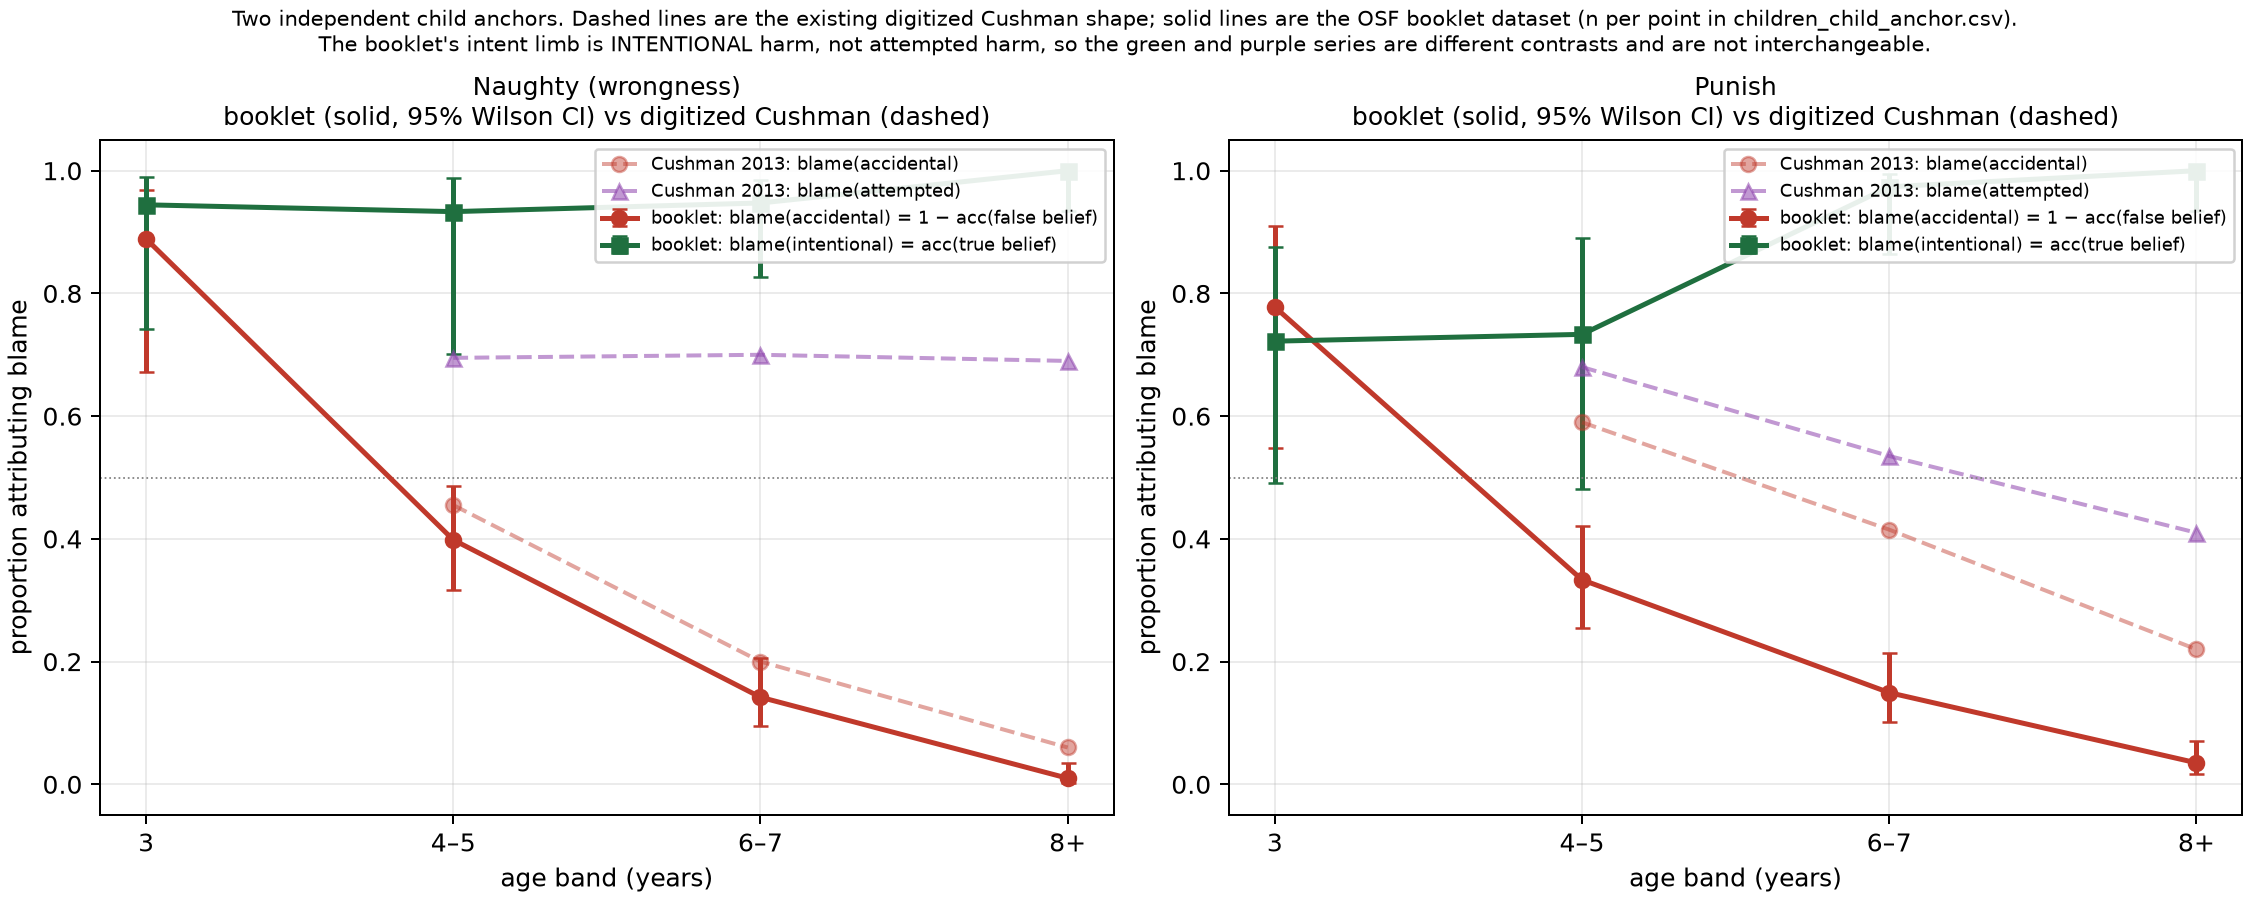
\includegraphics[width=\linewidth]{figures/child_anchor_booklet_vs_cushman.png}
    \caption{\textbf{Two independent child-reference shapes.}
    Solid lines are item-level booklet estimates with 95\% Wilson intervals; dashed lines are digitized Cushman series.
    The booklet contrast is intentional-minus-accidental and is not numerically interchangeable with the attempted-minus-accidental model contrast.}
    \label{fig:child-booklet}
\end{figure}

\subsection{Behavioral robustness and ancillary analyses}

\begin{table}[h]
\centering
\small
\caption{Supporting behavioral robustness results.}
\label{tab:behavior-robustness}
\begin{tabularx}{\textwidth}{@{}lXl@{}}
\toprule
Analysis & Result & Interpretation \\
\midrule
Common 1--7 prompts & 5/20 open models flip contrast sign & prompt sensitivity exists \\
Prompt construct variance & approximately 0\% in the project decomposition & wording/scale effects dominate construct label \\
EV versus sampling & correlation $>0.95$ for tested 7B instruct models & scoring parity supported in that slice \\
Qwen base$\rightarrow$instruct & mean paired shift approximately $-0.216$, paired $p\approx0.020$; Wilcoxon $p\approx0.063$ & family-specific evidence \\
Open scale versus contrast & Spearman $\rho\approx-0.23$, not significant & no scale claim \\
Source-scale agreement & pooled normalized correlation 0.71; bias $-0.06$; limits of agreement $[-0.44,+0.33]$ & cross-source averaging is imperfect \\
\bottomrule
\end{tabularx}
\end{table}

The two source instruments differ: the 2008 items use permissibility on a 1--3 scale and the 2009 items use blame on a 1--4 scale.
Normalization places both on a common condemnation direction but does not make the constructs identical.

\subsection{Measurement audits: normalization, clustering, story variance, and reliability}
\label{sec:supp-normalization}

The 2008 human scale (1 = forbidden, 3 = permissible) and the 2007 adult anchor run opposite to the model source-verbatim prompt; the 2009 (1--4 blame) and 2011 (1--7 wrongness) scales and all six factorial templates (1--7) share the model direction.
The mean of 11 open instruct models minus nine base models (2{,}000-resample scenario bootstraps) was $-0.319$ $[-0.345,-0.291]$ under endpoint scaling, $-0.309$ $[-0.334,-0.281]$ under per-model min--max, $-0.898$ SD $[-1.007,-0.786]$ under z-scores within model $\times$ template $\times$ source, and $-0.259$ $[-0.293,-0.225]$ under ranks; 9/9, 9/9, 7/9, and 8/9 pairs, respectively, were negative with intervals excluding zero.
Against endpoint scaling, the 34-entry model ordering had Spearman $\rho=0.996$, 0.945, and 0.946 with 0, 1, and 2 sign flips.
Under z-scores, the Qwen2.5-7B pair interval includes zero and Qwen2.5-14B reverses ($+0.19$ $[+0.03,+0.37]$), as it also does under ranks ($+0.05$ $[+0.005,+0.10]$); the ordering flips are OLMo-2-7B base and Gemini 2.5 Flash, both near zero under endpoint scaling.
Closed models enter the ordering without base partners, and Qwen chat-template-off reruns are separate entries excluded from class means.


\paragraph{Clustering and story variance.}
With Ward linkage and MDS on correlation distance between item rating profiles (20 models $\times$ 7 templates), outcome organized the item space (silhouette 0.30, adjusted Rand index 0.88), condition partly did (ARI 0.39), and intent (0.01, $\approx0$) and source (0.01, 0.07) did not; source clustering appeared only with the source-verbatim prompt (0.21, 0.22), where source and scale are confounded.
UMAP was not run.
Across the 20 open models, per-story variance in harm-outcome cells was about twice that of no-harm cells (accidental and intentional 0.081--0.087; attempted and neutral 0.036--0.043), and across-template variance was two to five times smaller (0.008--0.019).
In scenario-clustered regressions, accidental and intentional exceeded neutral by $+0.048$ ($p<10^{-4}$; $R^2=0.73$) and no clause-length term was significant (all $p>0.2$; across templates all $p>0.1$); the planned human-versus-model comparison was not run because the scanner data lack a story mapping.

\begin{table}[h]
\centering
\footnotesize
\caption{Spearman--Brown split-half reliability (median over 1{,}000 random splits; brackets are the 2.5--97.5\% split range). ``Within'' removes condition means first; model raters were z-scored within model $\times$ template $\times$ source.}
\label{tab:reliability}
\begin{tabular}{@{}lrrrr@{}}
\toprule
Raters & 2008 raw & 2008 within & 2009 within & 2011 within \\
\midrule
Templates (median of 20 models) & 0.94 & 0.89 & 0.92 & 0.93 \\
Instruct models (11) & 0.97 [0.95, 0.98] & 0.83 [0.76, 0.88] & 0.84 [0.77, 0.90] & 0.93 [0.83, 0.99] \\
Base models (9) & 0.59 [0.29, 0.68] & 0.36 [0.14, 0.52] & 0.59 [0.41, 0.72] & 0.64 [$-0.23$, 0.94] \\
MOR4 humans (13; story numbers) & 0.22 [$-0.31$, 0.56] & 0.39 [0.10, 0.61] & -- & -- \\
\bottomrule
\end{tabular}
\end{table}

The 2011 rows contain only ten items, and no per-item human data exist for 2009 or 2011.
The human row uses unmapped story numbers with roughly six raters per half (story $\times$ condition cells: 0.69 [0.59, 0.80]).
Closed-model sampled ratings were identical across the five samples for nearly all items, so sample-level split-half values are uninformative and are not interpreted.

\paragraph{MOR4 scanner behavior.}
The MOR4 files are a scanner replication of the 2008 design (18 subjects, up to six runs of eight trials); conditions recovered from SPM onsets matched the stored trial order in every session checked.
Five subjects recorded no responses and 314 of 792 trials (39.6\%) lack a response; only three response keys were used, matching the 1--3 scale of the 2008 appendix rather than the 1--4 mapping applied.
No story-to-scenario mapping was found, and the belief/outcome codes (T, G) and button direction were inferred from the data (the all-neutral cell had the lowest mean, SD 0.26).
Under that coding, means on the key-minus-48 scale for the two presentation levels coded BF and OF were 3.35/3.55 (intentional), 3.04/3.15 (attempted), 2.44/2.45 (accidental), and 2.03/2.11 (neutral); attempted minus accidental is $+0.60$ and $+0.70$, or about $+0.30$ and $+0.35$ if the keys are a 3-point scale.
These values are descriptive only and are not compared with model items.

\subsection{Story ablations and variance decomposition}
\label{sec:supp-ablation}

Ablated stories were scored with the seven factorial templates in Qwen2.5-7B and Llama-3.1-8B base and instruct models: agent's name only (298 stories), text before the foreshadowing sentence (298), belief sentences deleted (298), and text up to the outcome sentence (288).
Prior strength is $|$rating $-0.5|$ and context sensitivity is the full-story minus ablated rating (four models, 53 scenarios, scenario-bootstrap intervals).
Base/instruct mean prior strength was 0.17/0.23 (name only), 0.17/0.24 (before foreshadow), 0.17/0.26 (belief removed), and 0.15/0.16 (outcome removed); instruct minus base was $+0.056$ [0.050, 0.061], $+0.059$ [0.037, 0.082], $+0.083$ [0.065, 0.101], and $+0.007$ [$-0.003$, 0.018].
Mean absolute context sensitivity was 0.06/0.29, 0.05/0.28, 0.02/0.13, and 0.02/0.07, with instruct-minus-base differences of $+0.238$ [0.219, 0.255], $+0.228$ [0.201, 0.257], $+0.112$ [0.093, 0.134], and $+0.050$ [0.043, 0.057].


The first two ablations are identical across conditions, so their contrasts are zero by construction.
Removing the belief roughly doubled the instruct contrasts (Qwen $-0.24\rightarrow-0.45$; Llama $-0.20\rightarrow-0.47$); removing the outcome sentence while keeping the foreshadow halved them ($-0.10$, $-0.11$), leaving a harm effect of 0.15; base contrasts stayed within $\pm0.08$.
In a full-story decomposition over 20 open models, seven templates, and 298 stories ($R^2=0.49$), Type I shares in entry order were condition 17.3\%, condition $\times$ base/instruct 11.0\%, base/instruct 10.1\%, and at most 2.4\% for any other term; the largest unique $R^2$ drop was condition $\times$ base/instruct (8.6\%).
Main effects nested in interactions have zero unique drop, so their shares depend on entry order.

\subsection{Explicit ToM comparison}

The joint BigToM table in \cref{tab:bigtom-engaged} is the primary RQ1 result.
The following analyses are retained to prevent a confounded correlation from being overinterpreted:
\begin{itemize}[leftmargin=*]
    \item The raw all-model false-belief/contrast correlation is a confound demonstration because both variables proxy base/instruct status and model size.
    \item Instruct-only partial correlation: $r=-0.473$, 95\% interval $[-0.776,+0.513]$, $n=11$; uninformative.
    \item Covariate-adjusted OLS: partial $r=-0.310$, interval $[-0.612,+0.158]$; ToM coefficient $-0.379$, $p=0.211$.
    \item Within-family deltas: $r=-0.160$, interval $[-0.824,+0.807]$, $n=9$; uninformative.
    \item ToMi is not a primary ToM measure because 82\% of the scored slice was audited as non-ToM.
\end{itemize}

\paragraph{Standalone closed-model BigToM.}
The project also contains generative BigToM runs for closed models.
They are reported descriptively and are not pooled with the open log-probability protocol or used for a post-hoc correlation with the clean v3 moral reruns.

\begin{longtable}{@{}lrrrrl@{}}
\caption{Closed-model generative BigToM inventory. Partial and failed runs are retained visibly rather than imputed.}\label{tab:closed-bigtom}\\
\toprule
Model & $n$ & All & False belief & True belief & Status \\
\midrule
\endfirsthead
\toprule
Model & $n$ & All & False belief & True belief & Status \\
\midrule
\endhead
Claude Haiku 4.5 & 400 & 0.953 & 0.975 & 0.930 & complete \\
Claude Opus 4.6 & 400 & 0.985 & 0.985 & 0.985 & complete \\
Claude Opus 5 & 127 & 0.992 & 0.986 & 1.000 & partial \\
Claude Sonnet 4.6 & 400 & 0.940 & 0.990 & 0.890 & complete \\
Claude Sonnet 5 & 397 & 0.972 & 0.985 & 0.960 & partial \\
Gemini 2.5 Flash & 400 & 0.970 & 0.980 & 0.960 & complete \\
Gemini 2.5 Pro & 234 & 0.974 & 0.992 & 0.957 & partial \\
Gemini 3.5 Flash & 400 & 0.965 & 0.980 & 0.950 & complete \\
GPT-4o-mini & 400 & 0.915 & 0.955 & 0.875 & complete \\
GPT-4o & 400 & 0.968 & 0.970 & 0.965 & complete \\
GPT-5.4-mini & 400 & 0.950 & 0.990 & 0.910 & complete \\
GPT-5.5 & 393 & 0.990 & 0.990 & 0.990 & partial \\
o3 & 329 & 0.991 & 0.994 & 0.987 & partial \\
o4-mini & 373 & 0.984 & 0.995 & 0.972 & partial \\
Gemini 3.1 Pro preview & 0 & -- & -- & -- & failed \\
\bottomrule
\end{longtable}

\subsection{Post-training stages}

The full 11-row stage table is \cref{tab:stages}.
Stage shares are:
\begin{table}[h]
\centering
\small
\caption{Share of each family's base-to-final contrast shift.}
\label{tab:stage-shares}
\begin{tabular}{@{}lrrl@{}}
\toprule
Family & SFT share & Later-stage share & Dominant measured stage \\
\midrule
OLMo-2-7B & 85.4\% & 14.6\% & SFT \\
Tulu-3-8B & 65.4\% & 34.5\% & SFT \\
Zephyr-7B & 27.0\% & 73.0\% & DPO \\
\bottomrule
\end{tabular}
\end{table}

The ratio $\outcomebeta/\intentbeta$ spans 3.0--7.7 across all non-base stages.
Final-stage ratios are 6.6 for OLMo, 3.4 for Tulu, and 7.7 for Zephyr.
The robust statement is that outcome grows several-fold more than intent at each non-base stage; the exact multiplier is recipe-dependent.

\subsection{Linear probes and surface baselines}

\begin{table}[h]
\centering
\small
\caption{Probe ranges and span-matched baselines across the eight core open checkpoints.}
\label{tab:probe-summary}
\begin{tabular}{@{}lrrr@{}}
\toprule
Read position & Intent probe & Outcome probe & Relevant TF--IDF baseline \\
\midrule
Belief-clause endpoint & 0.900--0.983 & 0.793--0.924 & 0.591 intent; 0.581 outcome \\
Final story token & 0.671--0.883 & 0.980--1.000 & 0.594 intent; 0.755 outcome \\
\bottomrule
\end{tabular}
\end{table}

At the belief endpoint, all eight models have a larger probe-minus-surface gap for intent than outcome; the mean difference is $+0.0871$ (sign-test $p=0.0078$).
This was downgraded from a temporal-process headline after manual inspection showed that setup sentences can state the scenario's ground-truth hazard before the annotated belief clause.
The foreshadow analysis below localizes that information to a single sentence.
The result supports semantic generalization beyond bag-of-words, not anticipation of unseen content.
The table's TF--IDF values use all 298 rows; on the 290-story clause-masked set of the foreshadow analysis, the belief-endpoint outcome baselines are 0.631 (word) and 0.572 (character).

\subsection{Follow-up decoding: foreshadow, held-out templates, and token-wise}
\label{sec:supp-foreshadow}

\paragraph{Outcome at the intention stage.}
Main-text values for the 14 checkpoints use 290 stories after the clause mask and 1{,}000 permutations; the character TF--IDF baseline was 0.572, peak-layer belief-endpoint accuracy reached 0.92, and fixed-depth accuracy at the action endpoint was 0.62--0.83.
In token trajectories at the last belief token (288 2008/2009 stories), peak outcome accuracy on the original text was 0.71/0.80 for Llama-3.1-8B base/instruct (layer 16), 0.77/0.81 for OLMo-2-7B (layer 16), and 0.73/0.73 for Qwen2.5-7B (layers 22/14), against same-text TF--IDF of 0.60 (word) and 0.59 (character), all $p=0.001$.
Without the foreshadowing sentence, the text through the belief was byte-identical between outcome partners in 100\% of items, so chance accuracy is structural and no permutation test was run; trajectories were extracted without chat formatting at a fixed subset of depths.

\paragraph{Held-out templates.}
\label{sec:supp-templates}
Activations were taken at the last prompt token of each template, with chat formatting for both Qwen models and Llama-Instruct (Llama base has no chat template); OLMo was not extracted.
In construct-held-out splits the source-verbatim template stayed in training; all splits were crossed with scenario-grouped folds, and TF--IDF used the full prompt with the same splits.
Within-minus-pair gaps (about 0.10--0.20 beyond relative depth 0.6) exceeded within-minus-construct gaps.

\begin{table}[h]
\centering
\footnotesize
\caption{Intent decoding at the last prompt token. Fixed layer is relative depth 0.65; all accuracies have permutation $p=0.001$ (null mean 0.50, null 95th percentile $\leq0.53$). Word TF--IDF: within 0.602, pair 0.596, construct 0.600; character TF--IDF: 0.555, 0.550, 0.543.}
\label{tab:templates}
\begin{tabular}{@{}lrrrrrr@{}}
\toprule
Model & Layer & Within & Pair & Construct & Within $-$ constr.\ ($p$) & Peak constr.\ (layer) \\
\midrule
Qwen2.5-7B & 18 & 0.647 & 0.568 & 0.635 & 0.012 (0.15) & 0.755 (22) \\
Qwen2.5-7B-Instruct & 18 & 0.750 & 0.580 & 0.680 & 0.070 (0.001) & 0.825 (21) \\
Llama-3.1-8B & 21 & 0.698 & 0.560 & 0.601 & 0.097 (0.001) & 0.639 (17) \\
Llama-3.1-8B-Instruct & 21 & 0.859 & 0.706 & 0.801 & 0.058 (0.001) & 0.814 (27) \\
\bottomrule
\end{tabular}
\end{table}

\paragraph{Token-wise decoding.}
Eight stories failed the clause mask and ten had non-monotone stage ends, leaving 280 per model.
At the layers of \cref{fig:time-decoding}, the pre-specified statistics (1{,}000-resample scenario bootstraps; all intervals exclude zero) were: intent rise across the belief clause 0.37--0.44 (TF--IDF 0.13); intent change from the belief end to late bins $-0.16$ to $-0.21$ (TF--IDF 0.00); late intent slope $-0.011$ to $-0.015$ per bin; pre-outcome outcome slope $-0.004$ to $-0.010$ per bin; and outcome jump at the outcome clause 0.14--0.31 (TF--IDF 0.04).
In temporal generalization, the intent code formed a block over the belief and early action bins, whereas background-trained outcome codes transferred only weakly to the outcome clause, which formed a separate late block.
The RDM intent coefficient fell from 1.54--1.95 in the action stage to 0.25--0.37 in the outcome stage, a steeper decline than decoding accuracy; the two measure mean-pattern distance and linear separability, respectively.
An initial run coded the interaction RDM so that it summed to a constant with the intent and outcome RDMs, making the coefficients unidentifiable; it was recoded as a 0/1 conjunction (rank 3), all six models were rerun, and only corrected values are reported.

\subsection{Representation--behavior links}

\begin{table}[h]
\centering
\footnotesize
\caption{Tests linking representation to behavior.}
\label{tab:representation-links}
\begin{tabularx}{\textwidth}{@{}XrrrrX@{}}
\toprule
Analysis & Estimate & 95\% low & 95\% high & $n$ & Status \\
\midrule
Item-level primary slope & $+0.0619$ & $-0.1463$ & $+0.2701$ & 384 & informative null vs $+0.30$ \\
Item-level matched slope & $+0.0291$ & $-0.1649$ & $+0.2231$ & 424 & informative null vs $+0.30$ \\
RSA pair link & $+0.0980$ & $-0.3102$ & $+0.4596$ & 28 pairs & null \\
Model-level probe link & $\approx-0.209$ & $\approx-0.80$ & $\approx+0.58$ & $\approx8$ & uninformative; footnote only \\
\bottomrule
\end{tabularx}
\end{table}

The RSA test asks whether models with more similar internal geometry have more similar moral contrasts.
Its interval admits moderate effects in either direction, so it is described as a null in the tested sample rather than proof of no relation.

\subsection{E1 variance partition: undecidable}

The pre-registered E1 gate required lexical unique variance to remain below the intent/outcome hypothesis RDMs before factor-specific unique variance could be interpreted.
All 36 designated model--layer cells were excluded under the full-document control, and all 36 were again excluded under a span-matched setup-only control.
The experimental factors are lexically realized and setup text nearly identifies scenario, so lexical distance is neither an independent nuisance nor removable without also removing design information.
E1's P1 and P2 therefore have no verdict.
The post-hoc 3--18$\times$ outcome/intent ordering is not promoted to confirmatory evidence.

\subsection{E2 checkpoint-stage RSA: withdrawn for power}

Across six OLMo/Tulu stage transitions, cross-stage RDM shift and absolute contrast shift correlated at $\rho=+0.870$, with a cluster-bootstrap 95\% interval $[+0.200,+1.000]$.
Despite the high point estimate, $n=6$ was pre-specified as underpowered; P1 was withdrawn.
Withdrawal is not evidence for the converse.
A Spearman--Brown correction was required before comparing observed RSA with the split-half ceiling.

\subsection{Additive steering details}

\begin{table}[h]
\centering
\footnotesize
\caption{Causal steering summary at coherent doses.}
\label{tab:steering-summary}
\begin{tabularx}{\textwidth}{@{}Xrrrr@{}}
\toprule
Model & Baseline $\contrast$ & Intent-probe max $|\Delta|$ & Outcome control max $|\Delta|$ & Resolution ratio \\
\midrule
OLMo-2-7B-Instruct & $-0.4452$ & 0.0128 & 0.2319 & 18$\times$ \\
Qwen2.5-7B-Instruct & $-0.2667$ & 0.0155 & 0.2592 & 17$\times$ \\
\bottomrule
\end{tabularx}
\end{table}

Manipulation checks:
\begin{itemize}[leftmargin=*]
    \item For OLMo, downstream intent-decoding accuracy changed from 0.893 to 0.500; the probe-margin displacement was $-3.18$ SD and $\Delta\contrast=-0.0128$.
    \item For Qwen, downstream intent-decoding accuracy changed from 0.899 to 0.500; the probe-margin displacement was $+7.21$ SD and $\Delta\contrast=+0.0056$.
    \item Both coefficient signs drive decoding toward chance, indicating off-manifold displacement rather than selective strengthening in one direction.
    \item At shallow layers the outcome control is at the random-direction floor; those cells are uninformative.
    \item At peak-intent and deeper resolvable layers, the probe-weight intent direction remains at or near the random floor while the outcome direction is effective.
\end{itemize}

Difference-of-means ``intent'' directions can raise all four cell means.
Because the accidental cell begins closest to the top of the scale, it has least headroom; the diagonal contrast then moves through ceiling compression.
Those movements are not treated as selective intent reweighting.

\subsection{Prose/rating dissociation}

Models were asked to explain a rating without being prompted to mention belief, intent, or accident; mention was coded by a primary coder and was not randomized.

\begin{table}[h]
\centering
\small
\caption{Ratings restricted to stories whose explanation names belief or intent, primary coder.}
\label{tab:prose}
\begin{tabular}{@{}lrrrrr@{}}
\toprule
Model & Mention rate & $n$ subset & $\intentbeta$ & $\outcomebeta$ & Ratio \\
\midrule
OLMo-2-7B-Instruct & 0.815 & 243 & $+0.078$ & $+0.444$ & 5.7$\times$ \\
Qwen2.5-7B-Instruct & 0.691 & 206 & $+0.026$ & $+0.310$ & 12.2$\times$ \\
\bottomrule
\end{tabular}
\end{table}

Lexicon-coded mention rates were 0.859 and 0.711.
Lexicon--hand-label Cohen's $\kappa$ was 0.725--0.756; lexicon--LLM-coder $\kappa$ was 0.423--0.488.
Surface mention is not evidence that the mentioned state is correct or causally used, and explanations are post-hoc to the rating.

\subsection{Prompt curriculum}

\begin{table}[h]
\centering
\small
\caption{Pre-registered L5 prompt-curriculum change from baseline.}
\label{tab:curriculum}
\begin{tabular}{@{}lrrl@{}}
\toprule
Model & Baseline & L5 & $\Delta$ and bar \\
\midrule
Zephyr-7B & $-0.552$ & $-0.337$ & $+0.215$, met \\
Qwen2.5-14B-Instruct & $-0.338$ & $+0.004$ & $+0.342$, met \\
Tulu-3-8B & $-0.398$ & $-0.325$ & $+0.073$, not met \\
OLMo-2-7B-Instruct & $-0.687$ & $-0.434$ & $+0.253$, met \\
Mistral-7B-Instruct & $-0.460$ & $-0.397$ & $+0.063$, not met \\
Gemma-2-9B-Instruct & $-0.375$ & $-0.265$ & $+0.110$, not met \\
\bottomrule
\end{tabular}
\end{table}

The pre-registered success rule required at least four of six models to clear $+0.15$; three did.
At L5, five of six improvements were attributable primarily to reduced accidental condemnation.
In the secondary ablation, principle-alone exceeded the full stack by more than 0.05 in three of six models, and all models were sub-additive across components.
Intent-led attempted-cell increases appeared clearly in two of six models under principle-alone.

\subsection{Outcome erasure and control sequence}

\begin{table}[h]
\centering
\small
\caption{Gate-passing outcome-erasure results.}
\label{tab:erasure-summary}
\begin{tabular}{@{}lrrrl@{}}
\toprule
Model & $\Delta\contrast$ & Cell-spread retention & Outcome removed & Label \\
\midrule
OLMo-2-7B-Instruct & $+0.3182$ & 0.5124 & yes & recovery \\
Qwen2.5-7B-Instruct & $+0.2312$ & 0.6697 & yes & recovery \\
Tulu-3-8B & $+0.3480$ & 0.3753 & yes & collapse \\
\bottomrule
\end{tabular}
\end{table}

\paragraph{Original specificity test (E5a).}
The matched-norm Qwen scenario perturbation moved $\contrast$ by $+0.1345$ at perplexity ratio 1.60, exceeding both the 0.0988 effect floor and the 1.5 coherence bound.
The pre-specification did not restrict P1 to coherent doses, so P1 remains failed.
Outcome/nuisance separation was 10.26$\times$ in OLMo, 1.72$\times$ in Qwen, and 4.31$\times$ in Tulu; the 2$\times$ bar failed in Qwen.
At coherent doses only, the largest Qwen nuisance movement was $+0.0929$ and separation was 2.49$\times$, but this is a secondary restatement.

\paragraph{Orthogonalized erasure (E6).}
With nuisance directions orthogonalized against outcome and intent and dose restricted to $s\leq1$, the largest coherent nuisance movement was 0.0160.
Minimum model-wise separation was 9.9$\times$, 22.3$\times$, and 24.6$\times$.
E6's absolute-floor conjunction held in only one of three models because the matched outcome arm was scaled to approximately one-third to one-half strength while tested against a full-strength floor.
The ratio-based P2 held in all three.
E6 is a new control, not a reversal of E5a.

\paragraph{Symmetric residual control (E7b).}
At matched displacement:
\begin{itemize}[leftmargin=*]
    \item OLMo's scenario-orthogonal outcome arm moved $\contrast$ by $+0.1549$ and its full outcome control by $+0.1880$: A-shaped.
    \item Qwen's test arm moved $+0.0322$ and its positive control $+0.0630$, both below the 0.0988 floor: void.
    \item Tulu's test arm moved $+0.0941$, 95\% of the floor, while its positive control moved $+0.1420$ and its complement $+0.1008$: assigned to the pre-registered falsifier branch, but near the threshold.
\end{itemize}
The split authorizes no pooled outcome-specific claim.

\subsection{Cross-domain harm-code support}

The project-local Bruneau stimulus set uses 144 items in 72 matched pairs across physical pain, emotional suffering, and false-belief harm \citep{bruneau2012shared}.
Its local filename uses 2011, consistent with the article's December 2011 online publication; the journal issue and bibliography year are 2012.
It does not contain attempted-harm conditions and therefore cannot test intent weighting.
Within-domain harm decoding was often 0.9--1.0.
At a single selected layer per model, mean within-domain versus cross-domain decoding was 0.951 versus 0.771 for Qwen and 0.979 versus 0.809 for OLMo.
Substantial cross-domain transfer supports a largely shared harm representation while leaving the intent-use question open.

\subsection{Checkpoint emergence}

\begin{table}[h]
\centering
\small
\caption{End-of-trajectory RDM coefficients and behavioral engagement.}
\label{tab:e8-summary}
\begin{tabular}{@{}llrrl@{}}
\toprule
Family & Read position & $\beta_{\mathrm{intent}}$ & $\beta_{\mathrm{outcome}}$ & Gradeable checkpoints \\
\midrule
Pythia-1.4B & belief endpoint & $+0.1042$ & $+0.0003$ & 0/26 overall \\
Pythia-1.4B & story end & $-0.0065$ & $+0.4899$ & 0/26 overall \\
OLMo-2-7B & belief endpoint, depth .8 & $+0.108$ & $+0.010$ & 0/20 stage-1 \\
OLMo-2-7B & story end, depth .8 & $+0.021$ & $+0.494$ & 0/20 stage-1 \\
\bottomrule
\end{tabular}
\end{table}

Pythia details:
\begin{itemize}[leftmargin=*]
    \item 26 checkpoints, step 0 through 143{,}000.
    \item Step-0 gate passed: 0/20 intent/outcome predictor cells outside even the uncorrected 95\% band.
    \item The registered prediction that outcome would emerge before intent at the primary belief-endpoint cell failed; the cell was structurally unsuitable for that ordering test.
    \item The registered non-decreasing outcome-share prediction failed at the primary cell ($\rho=-0.639$, interval $[-0.935,-0.113]$).
    \item Shape verdicts across the primary specification were 17 smooth, two indistinguishable, and one breakpoint.
    \item Peak rating SD was 0.0859 against the 0.2191 floor.
\end{itemize}

OLMo details:
\begin{itemize}[leftmargin=*]
    \item 20 stage-1 revisions, steps 150 through 928{,}646.
    \item At the final stage-1 revision, the target/off-target pattern held at 5/5 belief-endpoint depths and 4/5 story-end depths; the replication criterion was at least 3/5 at each position.
    \item At depth 0.8, onset is bracketed between step 1{,}000 (approximately 5B tokens, inside null) and step 2{,}000 (approximately 9B tokens, clear).
    \item Sigmoid fits were preferred for belief-endpoint intent ($\Delta\mathrm{AICc}=5.504$, $R^2=0.9077$) and story-end outcome ($\Delta\mathrm{AICc}=30.988$, $R^2=0.9839$).
    \item No random-initialization checkpoint is published for this family.
    \item The joined trajectory has two seams: stage-1 activations were extracted in float32 while stage activations used float16, and stage-2 annealing is unsampled.
\end{itemize}

The Pythia and OLMo step indices are not directly comparable.
Approximate token counts place Pythia story-end outcome at approximately 2.1B tokens and belief-endpoint intent at approximately 6.3B, while OLMo brackets both at 5--9B.
Only order-of-magnitude similarity is claimed.

\subsection{Cross-cultural placement}
\label{sec:supp-crosscultural}

The cross-cultural comparison uses a different axis---intentional minus accidental at constant harm---because the ten-society dataset has no failed-attempt cell \citep{barrett2016societies,curtin2020kinship}.
Nine of ten societies had positive badness effects with intervals excluding zero; Yasawa was $0.0000$ [${-0.0265},+0.0227$].


\begin{table}[h]
\centering
\small
\caption{Badness intent effects at constant harm in ten societies.}
\label{tab:societies}
\begin{tabular}{@{}lrrr@{}}
\toprule
Society & $n$ subjects & Scaled effect & 95\% CI \\
\midrule
Storozhnitsa & 28 & $+0.2411$ & $[+0.1786,+0.3036]$ \\
Los Angeles & 39 & $+0.2115$ & $[+0.1282,+0.2949]$ \\
Sursurunga & 20 & $+0.2000$ & $[+0.0500,+0.3375]$ \\
Martu & 18 & $+0.1944$ & $[+0.0556,+0.3194]$ \\
Karo Batak & 30 & $+0.1833$ & $[+0.0833,+0.2917]$ \\
Hadza & 29 & $+0.1379$ & $[+0.0690,+0.2155]$ \\
Shuar & 34 & $+0.1324$ & $[+0.0072,+0.2574]$ \\
Himba & 24 & $+0.1146$ & $[+0.0417,+0.1979]$ \\
Tsimane & 32 & $+0.1016$ & $[+0.0156,+0.1955]$ \\
Yasawa & 66 & $+0.0000$ & $[-0.0265,+0.0227]$ \\
\bottomrule
\end{tabular}
\end{table}

The engaged-model count is 4/6 below the literal lowest society and 6/6 below the lowest society with a detectable positive effect.
For all 18 non-degenerate open models, the corresponding counts are 12/18 and 18/18.
The society intervals are over subjects, whereas deterministic model points have no commensurate subject-level uncertainty.

\subsection{Stimulus and measurement provenance}

The pre-repair parser appended rating prompts and parts of subsequent scenarios to selected harm cells.
Three counters must not be conflated: 144 regex-detector hits, 96 of 154 harm cells in the per-condition table, and 99 visible trailing artifacts in the archived CSV.
Repair changed 260 of 298 rows and recovered names/backgrounds for all 48 2008 scenarios.
An independently discovered CPR polarity inversion was corrected by deriving action polarity from text and audited manually.

Every pre-repair result was regenerated.
The project preserves a checksum-addressed contaminated master and quarantined outputs rather than deleting them.
The current validation script has ten hard checks and exits non-zero on failure.

Three measurement failures motivated the no-imputation rule:
\begin{enumerate}[leftmargin=*]
    \item a digit-token mapping failure that returned the scale midpoint;
    \item a coherence detector that rejected valid single-digit outputs; and
    \item a closed-API parser that wrote midpoint ratings for failed calls.
\end{enumerate}
A failed measurement is now missing and must carry an answer/parse status.

\subsection{Reproducibility boundaries}

Scenario-group bootstraps use 2{,}000 replicates and seed 0 in the shared resampler.
The item-level slope uses 10{,}000 item resamples; the ToM comparison uses 10{,}000 model resamples; RSA convergence uses 1{,}000 pair resamples.
The E6 rebuild reproduces the committed L40S outputs bit-exactly on matched hardware.
On A100 hardware, perplexity ratios differed by up to 0.031, contrast by at most 0.002, and no gate decision changed.

Raw activations are gitignored and must be regenerated.
Package-lock or container metadata sufficient to recreate the complete software environment is \missinginfo.
The public archival identifier for the clean closed v3 data is also \missinginfo.

\subsection{Excluded and incomplete measurements}

\begin{itemize}[leftmargin=*]
    \item Gemini-2.5-Pro closed behavioral run: partial; excluded.
    \item Closed reasoning-dose study: incomplete; no clean figure; excluded.
    \item Contaminated-era closed moral contrasts: quarantined; excluded.
    \item Stale combined open/closed ladder figures: excluded.
    \item ToMi primary comparison: excluded after slice-content audit.
    \item Missing coefficients at unengaged pretraining checkpoints: retained as missing, never plotted at zero.
\end{itemize}

\section{Claim Boundary Checklist}

The following formulations are licensed by the available evidence:
\begin{itemize}[leftmargin=*]
    \item ``Explicit false-belief success is insufficient evidence of applied intent use in the tested open models.''
    \item ``Intent is linearly decodable in the tested open checkpoints, while the tested representation--behavior links are null or uninformative.''
    \item ``Probe-weight intent steering is small relative to an outcome-direction positive control at resolvable depths in two models.''
    \item ``Outcome erasure produces the pre-registered recovery signature in two of three models.''
    \item ``SFT is sufficient in three public pipelines, while stage share is recipe-dependent.''
    \item ``Representational structure develops smoothly in the measured Pythia and OLMo trajectories; pretraining checkpoints are not behaviorally gradeable under this rating assay.''
    \item ``Intent decoding transfers to held-out rating constructs in two base/instruct pairs.''
    \item ``Outcome decodability at the belief endpoint reflects the foreshadowing sentence.''
\end{itemize}

The following formulations are not licensed:
\begin{itemize}[leftmargin=*]
    \item ``All LLMs fail intent-sensitive moral judgment.''
    \item ``No model reaches an eight-year-old level.''
    \item ``Outcome weighting is outside the human range.''
    \item ``The intent representation is causally inert at every layer or in every form.''
    \item ``Only the outcome direction controls judgment.''
    \item ``SFT rather than preference optimization causes the bias in every recipe.''
    \item ``The belief endpoint is outcome-free'' or ``the model predicts an unseen outcome.''
    \item ``The MOR4 scanner data provide an item-matched human reliability or variance benchmark.''
    \item ``Instruction tuning lowers the contrast in every model family'' or ``base and instruct models differ in template generalization in general.''
    \item ``Passing or matching behavior establishes genuine, conscious, or human-like ToM.''
\end{itemize}


\end{document}
